
% Default to the notebook output style

    


% Inherit from the specified cell style.




    
\documentclass[11pt]{article}

    
    
    \usepackage[T1]{fontenc}
    % Nicer default font (+ math font) than Computer Modern for most use cases
    \usepackage{mathpazo}

    % Basic figure setup, for now with no caption control since it's done
    % automatically by Pandoc (which extracts ![](path) syntax from Markdown).
    \usepackage{graphicx}
    % We will generate all images so they have a width \maxwidth. This means
    % that they will get their normal width if they fit onto the page, but
    % are scaled down if they would overflow the margins.
    \makeatletter
    \def\maxwidth{\ifdim\Gin@nat@width>\linewidth\linewidth
    \else\Gin@nat@width\fi}
    \makeatother
    \let\Oldincludegraphics\includegraphics
    % Set max figure width to be 80% of text width, for now hardcoded.
    \renewcommand{\includegraphics}[1]{\Oldincludegraphics[width=.8\maxwidth]{#1}}
    % Ensure that by default, figures have no caption (until we provide a
    % proper Figure object with a Caption API and a way to capture that
    % in the conversion process - todo).
    \usepackage{caption}
    \DeclareCaptionLabelFormat{nolabel}{}
    \captionsetup{labelformat=nolabel}

    \usepackage{adjustbox} % Used to constrain images to a maximum size 
    \usepackage{xcolor} % Allow colors to be defined
    \usepackage{enumerate} % Needed for markdown enumerations to work
    \usepackage{geometry} % Used to adjust the document margins
    \usepackage{amsmath} % Equations
    \usepackage{amssymb} % Equations
    \usepackage{textcomp} % defines textquotesingle
    % Hack from http://tex.stackexchange.com/a/47451/13684:
    \AtBeginDocument{%
        \def\PYZsq{\textquotesingle}% Upright quotes in Pygmentized code
    }
    \usepackage{upquote} % Upright quotes for verbatim code
    \usepackage{eurosym} % defines \euro
    \usepackage[mathletters]{ucs} % Extended unicode (utf-8) support
    \usepackage[utf8x]{inputenc} % Allow utf-8 characters in the tex document
    \usepackage{fancyvrb} % verbatim replacement that allows latex
    \usepackage{grffile} % extends the file name processing of package graphics 
                         % to support a larger range 
    % The hyperref package gives us a pdf with properly built
    % internal navigation ('pdf bookmarks' for the table of contents,
    % internal cross-reference links, web links for URLs, etc.)
    \usepackage{hyperref}
    \usepackage{longtable} % longtable support required by pandoc >1.10
    \usepackage{booktabs}  % table support for pandoc > 1.12.2
    \usepackage[inline]{enumitem} % IRkernel/repr support (it uses the enumerate* environment)
    \usepackage[normalem]{ulem} % ulem is needed to support strikethroughs (\sout)
                                % normalem makes italics be italics, not underlines
    

    
    
    % Colors for the hyperref package
    \definecolor{urlcolor}{rgb}{0,.145,.698}
    \definecolor{linkcolor}{rgb}{.71,0.21,0.01}
    \definecolor{citecolor}{rgb}{.12,.54,.11}

    % ANSI colors
    \definecolor{ansi-black}{HTML}{3E424D}
    \definecolor{ansi-black-intense}{HTML}{282C36}
    \definecolor{ansi-red}{HTML}{E75C58}
    \definecolor{ansi-red-intense}{HTML}{B22B31}
    \definecolor{ansi-green}{HTML}{00A250}
    \definecolor{ansi-green-intense}{HTML}{007427}
    \definecolor{ansi-yellow}{HTML}{DDB62B}
    \definecolor{ansi-yellow-intense}{HTML}{B27D12}
    \definecolor{ansi-blue}{HTML}{208FFB}
    \definecolor{ansi-blue-intense}{HTML}{0065CA}
    \definecolor{ansi-magenta}{HTML}{D160C4}
    \definecolor{ansi-magenta-intense}{HTML}{A03196}
    \definecolor{ansi-cyan}{HTML}{60C6C8}
    \definecolor{ansi-cyan-intense}{HTML}{258F8F}
    \definecolor{ansi-white}{HTML}{C5C1B4}
    \definecolor{ansi-white-intense}{HTML}{A1A6B2}

    % commands and environments needed by pandoc snippets
    % extracted from the output of `pandoc -s`
    \providecommand{\tightlist}{%
      \setlength{\itemsep}{0pt}\setlength{\parskip}{0pt}}
    \DefineVerbatimEnvironment{Highlighting}{Verbatim}{commandchars=\\\{\}}
    % Add ',fontsize=\small' for more characters per line
    \newenvironment{Shaded}{}{}
    \newcommand{\KeywordTok}[1]{\textcolor[rgb]{0.00,0.44,0.13}{\textbf{{#1}}}}
    \newcommand{\DataTypeTok}[1]{\textcolor[rgb]{0.56,0.13,0.00}{{#1}}}
    \newcommand{\DecValTok}[1]{\textcolor[rgb]{0.25,0.63,0.44}{{#1}}}
    \newcommand{\BaseNTok}[1]{\textcolor[rgb]{0.25,0.63,0.44}{{#1}}}
    \newcommand{\FloatTok}[1]{\textcolor[rgb]{0.25,0.63,0.44}{{#1}}}
    \newcommand{\CharTok}[1]{\textcolor[rgb]{0.25,0.44,0.63}{{#1}}}
    \newcommand{\StringTok}[1]{\textcolor[rgb]{0.25,0.44,0.63}{{#1}}}
    \newcommand{\CommentTok}[1]{\textcolor[rgb]{0.38,0.63,0.69}{\textit{{#1}}}}
    \newcommand{\OtherTok}[1]{\textcolor[rgb]{0.00,0.44,0.13}{{#1}}}
    \newcommand{\AlertTok}[1]{\textcolor[rgb]{1.00,0.00,0.00}{\textbf{{#1}}}}
    \newcommand{\FunctionTok}[1]{\textcolor[rgb]{0.02,0.16,0.49}{{#1}}}
    \newcommand{\RegionMarkerTok}[1]{{#1}}
    \newcommand{\ErrorTok}[1]{\textcolor[rgb]{1.00,0.00,0.00}{\textbf{{#1}}}}
    \newcommand{\NormalTok}[1]{{#1}}
    
    % Additional commands for more recent versions of Pandoc
    \newcommand{\ConstantTok}[1]{\textcolor[rgb]{0.53,0.00,0.00}{{#1}}}
    \newcommand{\SpecialCharTok}[1]{\textcolor[rgb]{0.25,0.44,0.63}{{#1}}}
    \newcommand{\VerbatimStringTok}[1]{\textcolor[rgb]{0.25,0.44,0.63}{{#1}}}
    \newcommand{\SpecialStringTok}[1]{\textcolor[rgb]{0.73,0.40,0.53}{{#1}}}
    \newcommand{\ImportTok}[1]{{#1}}
    \newcommand{\DocumentationTok}[1]{\textcolor[rgb]{0.73,0.13,0.13}{\textit{{#1}}}}
    \newcommand{\AnnotationTok}[1]{\textcolor[rgb]{0.38,0.63,0.69}{\textbf{\textit{{#1}}}}}
    \newcommand{\CommentVarTok}[1]{\textcolor[rgb]{0.38,0.63,0.69}{\textbf{\textit{{#1}}}}}
    \newcommand{\VariableTok}[1]{\textcolor[rgb]{0.10,0.09,0.49}{{#1}}}
    \newcommand{\ControlFlowTok}[1]{\textcolor[rgb]{0.00,0.44,0.13}{\textbf{{#1}}}}
    \newcommand{\OperatorTok}[1]{\textcolor[rgb]{0.40,0.40,0.40}{{#1}}}
    \newcommand{\BuiltInTok}[1]{{#1}}
    \newcommand{\ExtensionTok}[1]{{#1}}
    \newcommand{\PreprocessorTok}[1]{\textcolor[rgb]{0.74,0.48,0.00}{{#1}}}
    \newcommand{\AttributeTok}[1]{\textcolor[rgb]{0.49,0.56,0.16}{{#1}}}
    \newcommand{\InformationTok}[1]{\textcolor[rgb]{0.38,0.63,0.69}{\textbf{\textit{{#1}}}}}
    \newcommand{\WarningTok}[1]{\textcolor[rgb]{0.38,0.63,0.69}{\textbf{\textit{{#1}}}}}
    
    
    % Define a nice break command that doesn't care if a line doesn't already
    % exist.
    \def\br{\hspace*{\fill} \\* }
    % Math Jax compatability definitions
    \def\gt{>}
    \def\lt{<}
    % Document parameters
    \title{report\_notebook}
    
    
    

    % Pygments definitions
    
\makeatletter
\def\PY@reset{\let\PY@it=\relax \let\PY@bf=\relax%
    \let\PY@ul=\relax \let\PY@tc=\relax%
    \let\PY@bc=\relax \let\PY@ff=\relax}
\def\PY@tok#1{\csname PY@tok@#1\endcsname}
\def\PY@toks#1+{\ifx\relax#1\empty\else%
    \PY@tok{#1}\expandafter\PY@toks\fi}
\def\PY@do#1{\PY@bc{\PY@tc{\PY@ul{%
    \PY@it{\PY@bf{\PY@ff{#1}}}}}}}
\def\PY#1#2{\PY@reset\PY@toks#1+\relax+\PY@do{#2}}

\expandafter\def\csname PY@tok@w\endcsname{\def\PY@tc##1{\textcolor[rgb]{0.73,0.73,0.73}{##1}}}
\expandafter\def\csname PY@tok@c\endcsname{\let\PY@it=\textit\def\PY@tc##1{\textcolor[rgb]{0.25,0.50,0.50}{##1}}}
\expandafter\def\csname PY@tok@cp\endcsname{\def\PY@tc##1{\textcolor[rgb]{0.74,0.48,0.00}{##1}}}
\expandafter\def\csname PY@tok@k\endcsname{\let\PY@bf=\textbf\def\PY@tc##1{\textcolor[rgb]{0.00,0.50,0.00}{##1}}}
\expandafter\def\csname PY@tok@kp\endcsname{\def\PY@tc##1{\textcolor[rgb]{0.00,0.50,0.00}{##1}}}
\expandafter\def\csname PY@tok@kt\endcsname{\def\PY@tc##1{\textcolor[rgb]{0.69,0.00,0.25}{##1}}}
\expandafter\def\csname PY@tok@o\endcsname{\def\PY@tc##1{\textcolor[rgb]{0.40,0.40,0.40}{##1}}}
\expandafter\def\csname PY@tok@ow\endcsname{\let\PY@bf=\textbf\def\PY@tc##1{\textcolor[rgb]{0.67,0.13,1.00}{##1}}}
\expandafter\def\csname PY@tok@nb\endcsname{\def\PY@tc##1{\textcolor[rgb]{0.00,0.50,0.00}{##1}}}
\expandafter\def\csname PY@tok@nf\endcsname{\def\PY@tc##1{\textcolor[rgb]{0.00,0.00,1.00}{##1}}}
\expandafter\def\csname PY@tok@nc\endcsname{\let\PY@bf=\textbf\def\PY@tc##1{\textcolor[rgb]{0.00,0.00,1.00}{##1}}}
\expandafter\def\csname PY@tok@nn\endcsname{\let\PY@bf=\textbf\def\PY@tc##1{\textcolor[rgb]{0.00,0.00,1.00}{##1}}}
\expandafter\def\csname PY@tok@ne\endcsname{\let\PY@bf=\textbf\def\PY@tc##1{\textcolor[rgb]{0.82,0.25,0.23}{##1}}}
\expandafter\def\csname PY@tok@nv\endcsname{\def\PY@tc##1{\textcolor[rgb]{0.10,0.09,0.49}{##1}}}
\expandafter\def\csname PY@tok@no\endcsname{\def\PY@tc##1{\textcolor[rgb]{0.53,0.00,0.00}{##1}}}
\expandafter\def\csname PY@tok@nl\endcsname{\def\PY@tc##1{\textcolor[rgb]{0.63,0.63,0.00}{##1}}}
\expandafter\def\csname PY@tok@ni\endcsname{\let\PY@bf=\textbf\def\PY@tc##1{\textcolor[rgb]{0.60,0.60,0.60}{##1}}}
\expandafter\def\csname PY@tok@na\endcsname{\def\PY@tc##1{\textcolor[rgb]{0.49,0.56,0.16}{##1}}}
\expandafter\def\csname PY@tok@nt\endcsname{\let\PY@bf=\textbf\def\PY@tc##1{\textcolor[rgb]{0.00,0.50,0.00}{##1}}}
\expandafter\def\csname PY@tok@nd\endcsname{\def\PY@tc##1{\textcolor[rgb]{0.67,0.13,1.00}{##1}}}
\expandafter\def\csname PY@tok@s\endcsname{\def\PY@tc##1{\textcolor[rgb]{0.73,0.13,0.13}{##1}}}
\expandafter\def\csname PY@tok@sd\endcsname{\let\PY@it=\textit\def\PY@tc##1{\textcolor[rgb]{0.73,0.13,0.13}{##1}}}
\expandafter\def\csname PY@tok@si\endcsname{\let\PY@bf=\textbf\def\PY@tc##1{\textcolor[rgb]{0.73,0.40,0.53}{##1}}}
\expandafter\def\csname PY@tok@se\endcsname{\let\PY@bf=\textbf\def\PY@tc##1{\textcolor[rgb]{0.73,0.40,0.13}{##1}}}
\expandafter\def\csname PY@tok@sr\endcsname{\def\PY@tc##1{\textcolor[rgb]{0.73,0.40,0.53}{##1}}}
\expandafter\def\csname PY@tok@ss\endcsname{\def\PY@tc##1{\textcolor[rgb]{0.10,0.09,0.49}{##1}}}
\expandafter\def\csname PY@tok@sx\endcsname{\def\PY@tc##1{\textcolor[rgb]{0.00,0.50,0.00}{##1}}}
\expandafter\def\csname PY@tok@m\endcsname{\def\PY@tc##1{\textcolor[rgb]{0.40,0.40,0.40}{##1}}}
\expandafter\def\csname PY@tok@gh\endcsname{\let\PY@bf=\textbf\def\PY@tc##1{\textcolor[rgb]{0.00,0.00,0.50}{##1}}}
\expandafter\def\csname PY@tok@gu\endcsname{\let\PY@bf=\textbf\def\PY@tc##1{\textcolor[rgb]{0.50,0.00,0.50}{##1}}}
\expandafter\def\csname PY@tok@gd\endcsname{\def\PY@tc##1{\textcolor[rgb]{0.63,0.00,0.00}{##1}}}
\expandafter\def\csname PY@tok@gi\endcsname{\def\PY@tc##1{\textcolor[rgb]{0.00,0.63,0.00}{##1}}}
\expandafter\def\csname PY@tok@gr\endcsname{\def\PY@tc##1{\textcolor[rgb]{1.00,0.00,0.00}{##1}}}
\expandafter\def\csname PY@tok@ge\endcsname{\let\PY@it=\textit}
\expandafter\def\csname PY@tok@gs\endcsname{\let\PY@bf=\textbf}
\expandafter\def\csname PY@tok@gp\endcsname{\let\PY@bf=\textbf\def\PY@tc##1{\textcolor[rgb]{0.00,0.00,0.50}{##1}}}
\expandafter\def\csname PY@tok@go\endcsname{\def\PY@tc##1{\textcolor[rgb]{0.53,0.53,0.53}{##1}}}
\expandafter\def\csname PY@tok@gt\endcsname{\def\PY@tc##1{\textcolor[rgb]{0.00,0.27,0.87}{##1}}}
\expandafter\def\csname PY@tok@err\endcsname{\def\PY@bc##1{\setlength{\fboxsep}{0pt}\fcolorbox[rgb]{1.00,0.00,0.00}{1,1,1}{\strut ##1}}}
\expandafter\def\csname PY@tok@kc\endcsname{\let\PY@bf=\textbf\def\PY@tc##1{\textcolor[rgb]{0.00,0.50,0.00}{##1}}}
\expandafter\def\csname PY@tok@kd\endcsname{\let\PY@bf=\textbf\def\PY@tc##1{\textcolor[rgb]{0.00,0.50,0.00}{##1}}}
\expandafter\def\csname PY@tok@kn\endcsname{\let\PY@bf=\textbf\def\PY@tc##1{\textcolor[rgb]{0.00,0.50,0.00}{##1}}}
\expandafter\def\csname PY@tok@kr\endcsname{\let\PY@bf=\textbf\def\PY@tc##1{\textcolor[rgb]{0.00,0.50,0.00}{##1}}}
\expandafter\def\csname PY@tok@bp\endcsname{\def\PY@tc##1{\textcolor[rgb]{0.00,0.50,0.00}{##1}}}
\expandafter\def\csname PY@tok@fm\endcsname{\def\PY@tc##1{\textcolor[rgb]{0.00,0.00,1.00}{##1}}}
\expandafter\def\csname PY@tok@vc\endcsname{\def\PY@tc##1{\textcolor[rgb]{0.10,0.09,0.49}{##1}}}
\expandafter\def\csname PY@tok@vg\endcsname{\def\PY@tc##1{\textcolor[rgb]{0.10,0.09,0.49}{##1}}}
\expandafter\def\csname PY@tok@vi\endcsname{\def\PY@tc##1{\textcolor[rgb]{0.10,0.09,0.49}{##1}}}
\expandafter\def\csname PY@tok@vm\endcsname{\def\PY@tc##1{\textcolor[rgb]{0.10,0.09,0.49}{##1}}}
\expandafter\def\csname PY@tok@sa\endcsname{\def\PY@tc##1{\textcolor[rgb]{0.73,0.13,0.13}{##1}}}
\expandafter\def\csname PY@tok@sb\endcsname{\def\PY@tc##1{\textcolor[rgb]{0.73,0.13,0.13}{##1}}}
\expandafter\def\csname PY@tok@sc\endcsname{\def\PY@tc##1{\textcolor[rgb]{0.73,0.13,0.13}{##1}}}
\expandafter\def\csname PY@tok@dl\endcsname{\def\PY@tc##1{\textcolor[rgb]{0.73,0.13,0.13}{##1}}}
\expandafter\def\csname PY@tok@s2\endcsname{\def\PY@tc##1{\textcolor[rgb]{0.73,0.13,0.13}{##1}}}
\expandafter\def\csname PY@tok@sh\endcsname{\def\PY@tc##1{\textcolor[rgb]{0.73,0.13,0.13}{##1}}}
\expandafter\def\csname PY@tok@s1\endcsname{\def\PY@tc##1{\textcolor[rgb]{0.73,0.13,0.13}{##1}}}
\expandafter\def\csname PY@tok@mb\endcsname{\def\PY@tc##1{\textcolor[rgb]{0.40,0.40,0.40}{##1}}}
\expandafter\def\csname PY@tok@mf\endcsname{\def\PY@tc##1{\textcolor[rgb]{0.40,0.40,0.40}{##1}}}
\expandafter\def\csname PY@tok@mh\endcsname{\def\PY@tc##1{\textcolor[rgb]{0.40,0.40,0.40}{##1}}}
\expandafter\def\csname PY@tok@mi\endcsname{\def\PY@tc##1{\textcolor[rgb]{0.40,0.40,0.40}{##1}}}
\expandafter\def\csname PY@tok@il\endcsname{\def\PY@tc##1{\textcolor[rgb]{0.40,0.40,0.40}{##1}}}
\expandafter\def\csname PY@tok@mo\endcsname{\def\PY@tc##1{\textcolor[rgb]{0.40,0.40,0.40}{##1}}}
\expandafter\def\csname PY@tok@ch\endcsname{\let\PY@it=\textit\def\PY@tc##1{\textcolor[rgb]{0.25,0.50,0.50}{##1}}}
\expandafter\def\csname PY@tok@cm\endcsname{\let\PY@it=\textit\def\PY@tc##1{\textcolor[rgb]{0.25,0.50,0.50}{##1}}}
\expandafter\def\csname PY@tok@cpf\endcsname{\let\PY@it=\textit\def\PY@tc##1{\textcolor[rgb]{0.25,0.50,0.50}{##1}}}
\expandafter\def\csname PY@tok@c1\endcsname{\let\PY@it=\textit\def\PY@tc##1{\textcolor[rgb]{0.25,0.50,0.50}{##1}}}
\expandafter\def\csname PY@tok@cs\endcsname{\let\PY@it=\textit\def\PY@tc##1{\textcolor[rgb]{0.25,0.50,0.50}{##1}}}

\def\PYZbs{\char`\\}
\def\PYZus{\char`\_}
\def\PYZob{\char`\{}
\def\PYZcb{\char`\}}
\def\PYZca{\char`\^}
\def\PYZam{\char`\&}
\def\PYZlt{\char`\<}
\def\PYZgt{\char`\>}
\def\PYZsh{\char`\#}
\def\PYZpc{\char`\%}
\def\PYZdl{\char`\$}
\def\PYZhy{\char`\-}
\def\PYZsq{\char`\'}
\def\PYZdq{\char`\"}
\def\PYZti{\char`\~}
% for compatibility with earlier versions
\def\PYZat{@}
\def\PYZlb{[}
\def\PYZrb{]}
\makeatother


    % Exact colors from NB
    \definecolor{incolor}{rgb}{0.0, 0.0, 0.5}
    \definecolor{outcolor}{rgb}{0.545, 0.0, 0.0}



    
    % Prevent overflowing lines due to hard-to-break entities
    \sloppy 
    % Setup hyperref package
    \hypersetup{
      breaklinks=true,  % so long urls are correctly broken across lines
      colorlinks=true,
      urlcolor=urlcolor,
      linkcolor=linkcolor,
      citecolor=citecolor,
      }
    % Slightly bigger margins than the latex defaults
    
    \geometry{verbose,tmargin=1in,bmargin=1in,lmargin=1in,rmargin=1in}
    
    

    \begin{document}
    
    
    \maketitle
    
    

    
    \hypertarget{machine-learning-engineer-nanodegree}{%
\section{Machine Learning Engineer
Nanodegree}\label{machine-learning-engineer-nanodegree}}

\hypertarget{capstone-project}{%
\subsection{Capstone Project}\label{capstone-project}}

Victor São Paulo Ruela

February 5th, 2019

\hypertarget{i.-definition}{%
\subsection{I. Definition}\label{i.-definition}}

\hypertarget{project-overview}{%
\subsubsection{Project Overview}\label{project-overview}}

Partial Discharge (PD) signals are electrical discharges that can occur
inside the insulation of high voltage equipments. These signals have a
repetitive nature and are confined to small regions, which in the long
run can lead to irreparable damage to the equipment. Therefore, it is
vital for the energy industry companies to monitor the occcurrance of
PDs, in order to prevent accidents and guarantee a realiable energy
transmission for its customers.

Measuring these signals in the field is already very challenging task,
due to its low intensity and high noise levels from high voltage
systems. However, this is just one part of the problem: based on the
measurements, how can we predict some of its characteristics, such as
faults, the level of damage, local of occurrence and possible causes?
These are tasks that can be achieve with signal processing techniques
and machine learning algorithms.

The dataset that is going to be used is available from the VSB Power
Line Fault Detection Kaggle competition website:

https://www.kaggle.com/c/vsb-power-line-fault-detection

It contains several examples of labeled PD signals (fault or undamaged).
Each signal contains 800,000 measurements of a power line's voltage,
taken over 20 milliseconds for each one of the three phases.

\hypertarget{problem-statement}{%
\subsubsection{Problem Statement}\label{problem-statement}}

The goal is to train a classification algorithm to predict for PD signal
measurements if a power line damaged or not. I will be tackling this
problem as a binary classification problem, also applying digital signal
processing techniques to extract the most relevant features from the PD
signals.

The first task will be to apply signal processing techniques in order to
remove the background noise from the measurements and obtain a clear
representation of the partial discharge signals. This can be done using
digital filters (Butterworth, Chebyschev, etc.), the Fourier Transform
and the Discrete Wavelet Transform (DWT). After that, new features will
be extracted, such as amount of PDs and the frequency-domain content. If
necessary, more features can be include based on the thesis from the
competition's responsible {[}1{]}.

For the training models, I pretend to compare binary classification
models, such as Logistic Regression and Random Forests. I will work with
simpler models in order to have more time available for the feature
extraction, since this should be the most important taks on this
porject. I expect to spend 70\% of the time on the signal processing and
feature extraction parts and 30\% of the time on training models and
tweaking parameters.

\hypertarget{metrics}{%
\subsubsection{Metrics}\label{metrics}}

The results will be evaluated with the
\href{https://en.wikipedia.org/wiki/Matthews_correlation_coefficient}{Matthews
correlation coefficient (MCC)} between the predicted and the observed
response:

\begin{figure}
\centering
\includegraphics{https://wikimedia.org/api/rest_v1/media/math/render/svg/5caa90fc15105b74b59a30bbc9cc2e5bd43a13b7}
\caption{alt text}
\end{figure}

where TP is the number of true positives, TN the number of true
negatives, FP the number of false positives, and FN the number of false
negatives. This is a very suitable metric, since the dataset is probably
unbalanced because faults are not very frequent.

This is the same metric used in the competition.

    \hypertarget{ii.-analysis}{%
\subsection{II. Analysis}\label{ii.-analysis}}

\hypertarget{data-exploration-and-visualization}{%
\subsubsection{Data Exploration and
Visualization}\label{data-exploration-and-visualization}}

The dataset is available at
https://www.kaggle.com/c/vsb-power-line-fault-detection/data

It contains the following files:

\begin{enumerate}
\def\labelenumi{\alph{enumi})}
\tightlist
\item
  metadata\_{[}train/test{]}.csv - The signal general information and
  labels. Contatins the following columns:
\end{enumerate}

\begin{itemize}
\item
  \texttt{id\_measurement}: the ID code for a trio of signals recorded
  at the same time.
\item
  \texttt{signal\_id}: the foreign key for the signal data. Each signal
  ID is unique across both train and test, so the first ID in train is
  `0' but the first ID in test is `8712'.
\item
  \texttt{phase}: the phase ID code within the signal trio. The phases
  may or may not all be impacted by a fault on the line.
\item
  \texttt{target}: 0 if the power line is undamaged, 1 if there is a
  fault.
\end{itemize}

\begin{enumerate}
\def\labelenumi{\alph{enumi})}
\setcounter{enumi}{1}
\tightlist
\item
  {[}train/test{]}.parquet - The signal data. Each column contains one
  signal; 800,000 int8 measurements as exported with pyarrow.parquet
  version 0.11. More information about the parquet format can be found
  in https://acadgild.com/blog/parquet-file-format-hadoop.
\end{enumerate}

The metadata file is the link between the actual PD signals measurements
in the parquet file and its label. For example, to access the signal
with ID ``1'', you just need to load the column ``1'' from the .parquet
file. This is actually a very interesting feature, because it allows to
optimize the memory consumption by processing one signal at a time.

The \texttt{metadata\_train.csv} file contains \texttt{8712} rows, each
one representing a signal available in the \texttt{train.parquet} file.
The overall and per phase distribution for the labels are displayed in
the figures below.

\begin{figure}
\centering
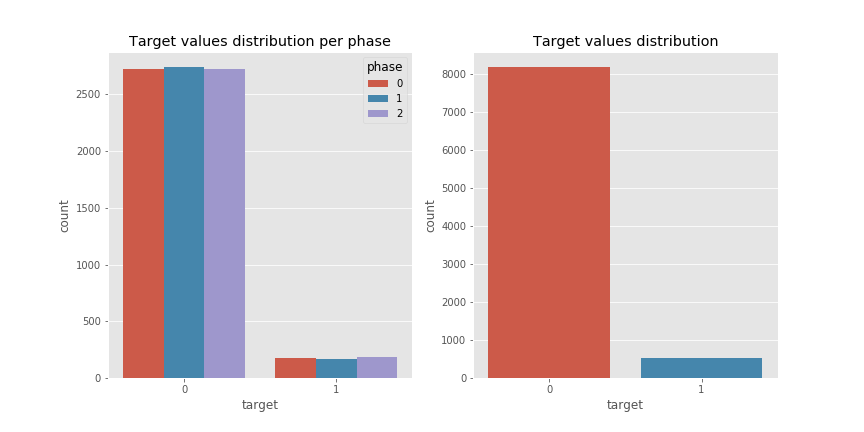
\includegraphics{train_data_dist_twosided.png}
\caption{Label distribution - Overall}
\end{figure}

We can clearly see the data is very unbalanced: only \texttt{6.0262\%}
of the data contains examples of fault signals. This was expected, since
a fault event is not very common. Looking at the distribution
considering the phase of the signal, we can see that the labels are
evenly distributed among them. Therefore, phase should not be an input
variable to the models, since it won't add any relevante information.

Eah signal in the \texttt{train.parquet} contains \texttt{800,000}
measurements of a power line's voltage, taken over \texttt{20}
milliseconds. Thefore, the sampling rate is \texttt{40Mhz}. A sample
signal PD signal for each phase can be seen in the figure below.

\begin{figure}
\centering
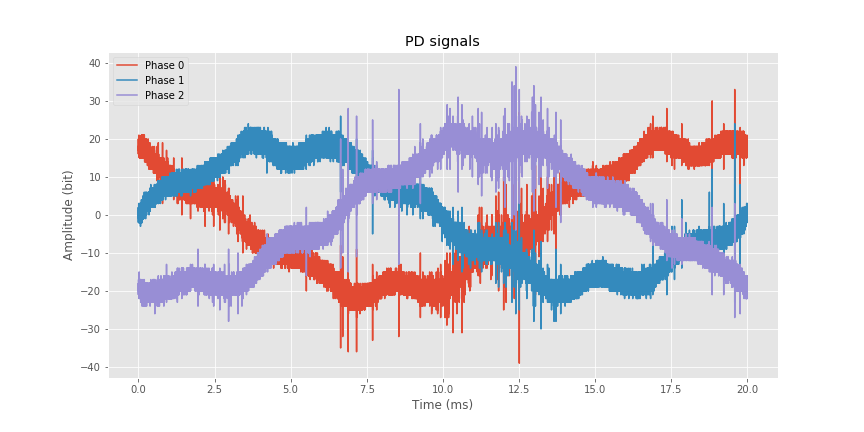
\includegraphics{signal_phase_example.png}
\caption{PD Signal}
\end{figure}

The figure below shows a comparison between a fault and normal example
signals. 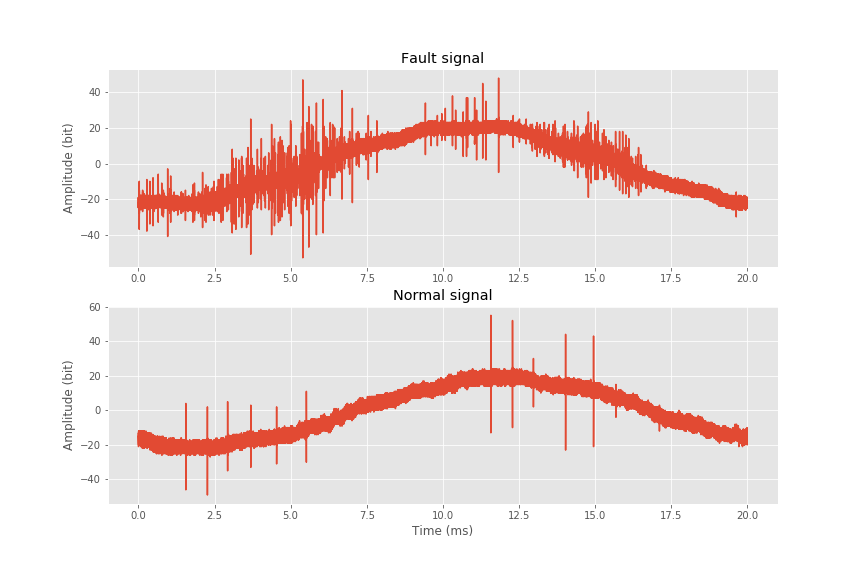
\includegraphics{signal_fault_normal_raw.png}

Based on these examples, the following can be inferred about PD signals:

\begin{itemize}
\tightlist
\item
  There is a lot of background noise, which can be incorrectly
  identified as a PD pattern. Therefore, it is necessary to denoise this
  signal ass the first step for the analysis.
\item
  It's not easy to visually observe an actual PD pattern, since it
  happens very fast.
\item
  The start and end of the measuremente cycle is different depending on
  the phase.
\end{itemize}

Moreover, the raw time-based data format should not be used for the
machine learning algorithms, since this would lead to have
\texttt{800,000} features as inputs to the model.Therefore, signal
processing techniques will have to applied to extract features that can
accurately represent the signal.

\hypertarget{algorithms-and-techniques}{%
\subsubsection{Algorithms and
Techniques}\label{algorithms-and-techniques}}

The following classifiers will be teste and the one with the highest
cross-validation score on the dataset will be chosen:
\href{https://scikit-learn.org/stable/modules/generated/sklearn.linear_model.LogisticRegression.html}{Logistic
Regression},
\href{https://scikit-learn.org/stable/modules/generated/sklearn.neighbors.KNeighborsClassifier.html}{kNN},
\href{https://scikit-learn.org/stable/modules/generated/sklearn.ensemble.RandomForestClassifier.html}{Random
Forest} and
\href{https://scikit-learn.org/stable/modules/generated/sklearn.ensemble.GradientBoostingClassifier.html}{Gradient
Boosting}. They are well known techniques for the binary classification
task and are expected to perform well on this dataset, since they do not
require very large datasets to work. They will be evaluated with their
default pararemeters, as described in their documentation page.

The chosen model will use as inputs the features extracted from the raw
PD signals and the respective labels (see the
\texttt{Data\ Preprocessing} section). A grid search will be executed in
order to tune its hyperparameters and find the optimal classifier. For
example, for the Random Forest, the following hyperparameters can be
optimized:

\begin{itemize}
\tightlist
\item
  \texttt{n\_estimators}: The number of trees in the forest
\item
  \texttt{max\_features}: The number of features to consider when
  looking for the best split:
\item
  \texttt{max\_depth}: The maximum depth of the tree
\item
  \texttt{min\_samples\_split}: The minimum number of samples required
  to split an internal node
\item
  \texttt{min\_samples\_leaf}: The minimum number of samples required to
  be at a leaf node
\end{itemize}

\hypertarget{benchmark}
accuracy. This model will also have a baseline value of \texttt{0.0} for
the Mathews Correlation Coefficient.

    \hypertarget{iii.-methodology}{%
\subsection{III. Methodology}\label{iii.-methodology}}

\hypertarget{data-preprocessing}{%
\subsubsection{Data Preprocessing}\label{data-preprocessing}}

\hypertarget{feature-extraction}{%
\paragraph{Feature Extraction}\label{feature-extraction}}

As discussed in the previous sections, signal processing techniques must
be applied in order to extract the most relevant information from the
signals. The first step is applying a filter to the signal in order to
remove the background noise. An analysis of the most common PD denoising
techniques is available in {[}2{]}. For this project, a high pass filter
and a Discrete Wavelet Transform (DWT) denoising technique will be used.

The high pass filter will remove all frequency content below a certain
threshold. This is very important to remove the 50Hz baseline frequency
from the power line, and also some low frequency noise. The threshold
that is going to be used is 10kHz, since PD patterns are only observed
above this value.

The DWT is the most used signal processing technique for PD denoising,
having several papers studying its application available in the
literature. It works by decomposing the signal in several scales and
levels based on a pre-selected mother Wavelet. The framework for PD
denoising consists in:

\begin{itemize}
\tightlist
\item
  Apply the DWT to the noisy signal until a decomposition level where
  its possible to distinguish the DP signal. This will calculate the
  wavelet coefficients \(c\) for each level.
\item
  Chosse an appropriate threshold \(T_{d}\) for selecting the
  coefficients for each level. This can be done either with soft or hard
  thresholding.
\item
  Recover the denoised signal using the inverse discrete Wavelet
  transform from the coefficients selected previously.
\end{itemize}

A more detailed description regarding the Wavelet denoising framework
can be found in {[}1,3{]}. For this project, the a hard-thresholding
approach from {[}1{]} will be used. The limit \(T_{d,j}\) is calculated
based on the Mean Absolute Deviation (MAD), using the following
equations:

\[\sigma = \frac{1}{0.6745}~MAD(|c|) \]

\[T_{d} = \sigma\sqrt{2\log{n}} \]

where \(n\) is the lenght of the signal. The selected mother wavelet
will be the \texttt{Debauchy\ 4}, since it was indicated in {[}2{]} as
the most similar to the PD pattern.

The high pass filter and DWT denoising will be applied for every signal
in the database. After this step, we can start extracting new features
to represente this signal. An filtered signal example can be seen in the
figure below.

\begin{figure}
\centering
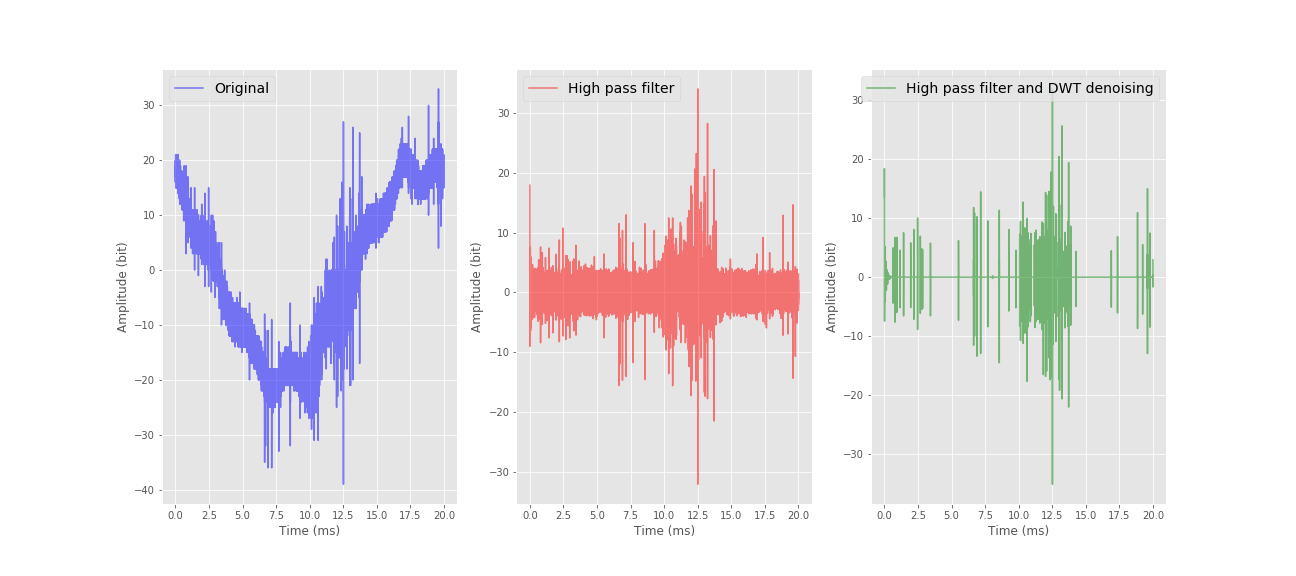
\includegraphics{signal_phase_denoised.png}
\caption{PD Signal Denoised}
\end{figure}

Afther that, time and frequency domain features will be extracted from
the denoised signal. According to {[}4{]}, the most relevant time domain
features are:

\begin{itemize}
\tightlist
\item
  Number of peaks
\item
  Mean width of peaks
\item
  Max width of peaks
\item
  Min width of peaks
\item
  Mean height of peaks
\item
  Max height of peaks
\item
  Min height of peaks
\end{itemize}

The signal will be divided into 4 sections of size \texttt{200,000} and
these features will be extracted for each subset, as suggested in
{[}4{]}. This is done because the appearance of peaks are not random,
i.e, they are clustered in specific subparts of the sinusoidal signal.
This yields a total of 28 features extracted.

In order to extract these features, the functions
\href{https://docs.scipy.org/doc/scipy/reference/generated/scipy.signal.find_peaks.html}{find\_peaks}
and
\href{https://docs.scipy.org/doc/scipy/reference/generated/scipy.signal.peak_widths.html\#scipy.signal.peak_widths}{peak\_widths}
from the \texttt{scipy} package will be used. It was necessary to fine
tune the input parameters for both functions, and after several trials
the following parameters were selected:

\begin{enumerate}
\def\labelenumi{\arabic{enumi}.}
\tightlist
\item
  \textbf{find\_peaks}

  \begin{itemize}
  \item
    prominence: \texttt{10} (The prominence of a peak measures how much
    a peak stands out from the surrounding baseline of the signal and is
    defined as the vertical distance between the peak and its lowest
    contour line.)
  \item
    distance: \texttt{50} (Required minimal horizontal distance in
    samples between neighbouring peaks)
  \end{itemize}
\item
  \textbf{peak\_widths}

  \begin{itemize}
  \tightlist
  \item
    rel\_height: \texttt{0.9} (Relative height at which the peak width
    is measured as a percentage of its prominence)
  \end{itemize}
\end{enumerate}

In the following figures, it is possible to see the peaks from an
example signal and also have a closer look at the width and height of a
peak.

\begin{figure}
\centering
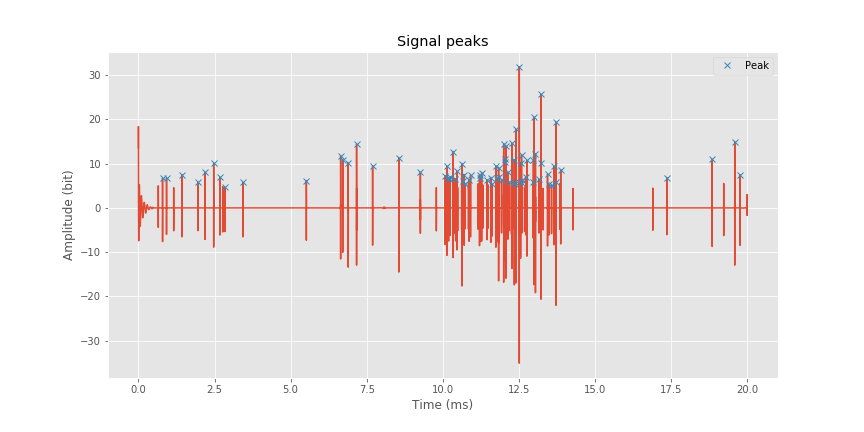
\includegraphics{signal_peaks.png}
\caption{Signal Peaks}
\end{figure}

\begin{figure}
\centering
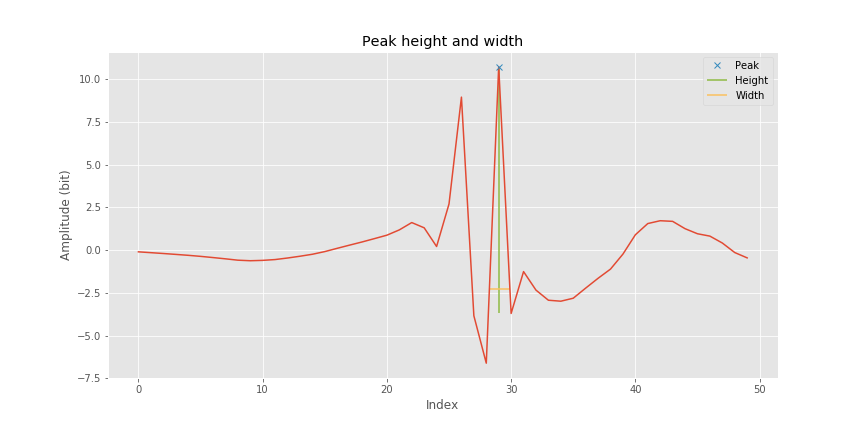
\includegraphics{signal_peak_zoom.png}
\caption{Peak height and width}
\end{figure}

The frequency domain features are based on the power spectral density
(PSD) of each denoised signal. The PSD will not be calculated based on
the raw signal because the noise contamination in higher frequencies
will introduce undesired bias to the data. The PSD will be split into 4
equals sections of 5 MHz (Nyquist frequency divided by 4), such that we
can extract the following features from the signal at different
frequency ranges:

\begin{itemize}
\tightlist
\item
  Sum of power spectrum
\item
  Maximum value
\item
  Mean value
\end{itemize}

This will be calculated with the
\href{https://docs.scipy.org/doc/scipy-0.14.0/reference/generated/scipy.signal.welch.html}{welch}
function from the \texttt{scipy} package. Welch's method calculates an
estimate of the power spectral density by dividing the data into
overlapping segments, computing a modified periodogram for each segment
and averaging the periodograms. An example for a faulted and normal
signal can be seen in the figure below. This task yields more 16
extracted features.

\begin{figure}
\centering
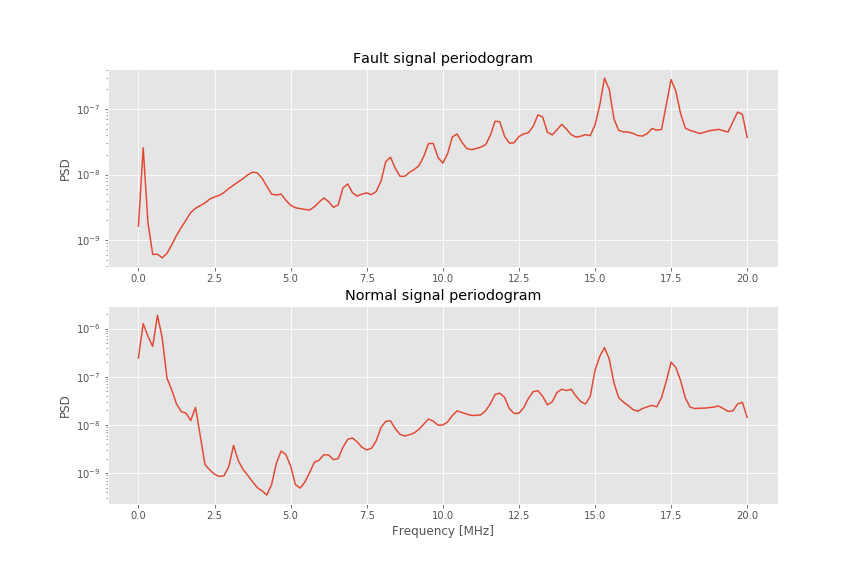
\includegraphics{signal_fault_normal_psd_denoised.png}
\caption{Power spectral density}
\end{figure}

After applying these two feature extraction, we finally have the dataset
that is going to be used for training our prediction models. This
dataset has 40 numerical features for each signal and their
corresponding labels.

\hypertarget{feature-transformation}{%
\paragraph{Feature Transformation}\label{feature-transformation}}

The statistical description can be seen in the table below.

\begin{longtable}[]{@{}llllllll@{}}
\toprule
\begin{minipage}[b]{0.16\columnwidth}\raggedright
Feature\strut
\end{minipage} & \begin{minipage}[b]{0.09\columnwidth}\raggedright
mean\strut
\end{minipage} & \begin{minipage}[b]{0.09\columnwidth}\raggedright
std\strut
\end{minipage} & \begin{minipage}[b]{0.09\columnwidth}\raggedright
min\strut
\end{minipage} & \begin{minipage}[b]{0.09\columnwidth}\raggedright
25\%\strut
\end{minipage} & \begin{minipage}[b]{0.09\columnwidth}\raggedright
50\%\strut
\end{minipage} & \begin{minipage}[b]{0.09\columnwidth}\raggedright
75\%\strut
\end{minipage} & \begin{minipage}[b]{0.08\columnwidth}\raggedright
max\strut
\end{minipage}\tabularnewline
\midrule
\endhead
\begin{minipage}[t]{0.16\columnwidth}\raggedright
number\_of\_peaks\_p1\strut
\end{minipage} & \begin{minipage}[t]{0.09\columnwidth}\raggedright
3.282633e+01\strut
\end{minipage} & \begin{minipage}[t]{0.09\columnwidth}\raggedright
7.949112e+01\strut
\end{minipage} & \begin{minipage}[t]{0.09\columnwidth}\raggedright
0.000000e+00\strut
\end{minipage} & \begin{minipage}[t]{0.09\columnwidth}\raggedright
3.000000e+00\strut
\end{minipage} & \begin{minipage}[t]{0.09\columnwidth}\raggedright
1.000000e+01\strut
\end{minipage} & \begin{minipage}[t]{0.09\columnwidth}\raggedright
3.000000e+01\strut
\end{minipage} & \begin{minipage}[t]{0.08\columnwidth}\raggedright
1144.000000\strut
\end{minipage}\tabularnewline
\begin{minipage}[t]{0.16\columnwidth}\raggedright
number\_of\_peaks\_p2\strut
\end{minipage} & \begin{minipage}[t]{0.09\columnwidth}\raggedright
3.183942e+01\strut
\end{minipage} & \begin{minipage}[t]{0.09\columnwidth}\raggedright
8.018707e+01\strut
\end{minipage} & \begin{minipage}[t]{0.09\columnwidth}\raggedright
0.000000e+00\strut
\end{minipage} & \begin{minipage}[t]{0.09\columnwidth}\raggedright
2.000000e+00\strut
\end{minipage} & \begin{minipage}[t]{0.09\columnwidth}\raggedright
9.000000e+00\strut
\end{minipage} & \begin{minipage}[t]{0.09\columnwidth}\raggedright
2.700000e+01\strut
\end{minipage} & \begin{minipage}[t]{0.08\columnwidth}\raggedright
1164.000000\strut
\end{minipage}\tabularnewline
\begin{minipage}[t]{0.16\columnwidth}\raggedright
number\_of\_peaks\_p3\strut
\end{minipage} & \begin{minipage}[t]{0.09\columnwidth}\raggedright
3.176102e+01\strut
\end{minipage} & \begin{minipage}[t]{0.09\columnwidth}\raggedright
7.946652e+01\strut
\end{minipage} & \begin{minipage}[t]{0.09\columnwidth}\raggedright
0.000000e+00\strut
\end{minipage} & \begin{minipage}[t]{0.09\columnwidth}\raggedright
2.000000e+00\strut
\end{minipage} & \begin{minipage}[t]{0.09\columnwidth}\raggedright
9.000000e+00\strut
\end{minipage} & \begin{minipage}[t]{0.09\columnwidth}\raggedright
2.800000e+01\strut
\end{minipage} & \begin{minipage}[t]{0.08\columnwidth}\raggedright
1155.000000\strut
\end{minipage}\tabularnewline
\begin{minipage}[t]{0.16\columnwidth}\raggedright
number\_of\_peaks\_p4\strut
\end{minipage} & \begin{minipage}[t]{0.09\columnwidth}\raggedright
3.221247e+01\strut
\end{minipage} & \begin{minipage}[t]{0.09\columnwidth}\raggedright
8.259928e+01\strut
\end{minipage} & \begin{minipage}[t]{0.09\columnwidth}\raggedright
0.000000e+00\strut
\end{minipage} & \begin{minipage}[t]{0.09\columnwidth}\raggedright
2.000000e+00\strut
\end{minipage} & \begin{minipage}[t]{0.09\columnwidth}\raggedright
9.000000e+00\strut
\end{minipage} & \begin{minipage}[t]{0.09\columnwidth}\raggedright
2.800000e+01\strut
\end{minipage} & \begin{minipage}[t]{0.08\columnwidth}\raggedright
1146.000000\strut
\end{minipage}\tabularnewline
\begin{minipage}[t]{0.16\columnwidth}\raggedright
mean\_width\_of\_peaks\_p1\strut
\end{minipage} & \begin{minipage}[t]{0.09\columnwidth}\raggedright
8.630635e-04\strut
\end{minipage} & \begin{minipage}[t]{0.09\columnwidth}\raggedright
1.748492e-03\strut
\end{minipage} & \begin{minipage}[t]{0.09\columnwidth}\raggedright
0.000000e+00\strut
\end{minipage} & \begin{minipage}[t]{0.09\columnwidth}\raggedright
7.329588e-05\strut
\end{minipage} & \begin{minipage}[t]{0.09\columnwidth}\raggedright
2.927462e-04\strut
\end{minipage} & \begin{minipage}[t]{0.09\columnwidth}\raggedright
8.171508e-04\strut
\end{minipage} & \begin{minipage}[t]{0.08\columnwidth}\raggedright
0.019447\strut
\end{minipage}\tabularnewline
\begin{minipage}[t]{0.16\columnwidth}\raggedright
mean\_width\_of\_peaks\_p2\strut
\end{minipage} & \begin{minipage}[t]{0.09\columnwidth}\raggedright
8.074817e-04\strut
\end{minipage} & \begin{minipage}[t]{0.09\columnwidth}\raggedright
1.542744e-03\strut
\end{minipage} & \begin{minipage}[t]{0.09\columnwidth}\raggedright
0.000000e+00\strut
\end{minipage} & \begin{minipage}[t]{0.09\columnwidth}\raggedright
4.746766e-05\strut
\end{minipage} & \begin{minipage}[t]{0.09\columnwidth}\raggedright
3.000340e-04\strut
\end{minipage} & \begin{minipage}[t]{0.09\columnwidth}\raggedright
8.291256e-04\strut
\end{minipage} & \begin{minipage}[t]{0.08\columnwidth}\raggedright
0.019327\strut
\end{minipage}\tabularnewline
\begin{minipage}[t]{0.16\columnwidth}\raggedright
mean\_width\_of\_peaks\_p4\strut
\end{minipage} & \begin{minipage}[t]{0.09\columnwidth}\raggedright
7.308763e-04\strut
\end{minipage} & \begin{minipage}[t]{0.09\columnwidth}\raggedright
1.456980e-03\strut
\end{minipage} & \begin{minipage}[t]{0.09\columnwidth}\raggedright
0.000000e+00\strut
\end{minipage} & \begin{minipage}[t]{0.09\columnwidth}\raggedright
4.004865e-05\strut
\end{minipage} & \begin{minipage}[t]{0.09\columnwidth}\raggedright
2.600330e-04\strut
\end{minipage} & \begin{minipage}[t]{0.09\columnwidth}\raggedright
7.639245e-04\strut
\end{minipage} & \begin{minipage}[t]{0.08\columnwidth}\raggedright
0.018890\strut
\end{minipage}\tabularnewline
\begin{minipage}[t]{0.16\columnwidth}\raggedright
mean\_width\_of\_peaks\_p3\strut
\end{minipage} & \begin{minipage}[t]{0.09\columnwidth}\raggedright
5.046811e-04\strut
\end{minipage} & \begin{minipage}[t]{0.09\columnwidth}\raggedright
1.226370e-03\strut
\end{minipage} & \begin{minipage}[t]{0.09\columnwidth}\raggedright
0.000000e+00\strut
\end{minipage} & \begin{minipage}[t]{0.09\columnwidth}\raggedright
2.521847e-05\strut
\end{minipage} & \begin{minipage}[t]{0.09\columnwidth}\raggedright
1.673808e-04\strut
\end{minipage} & \begin{minipage}[t]{0.09\columnwidth}\raggedright
4.927585e-04\strut
\end{minipage} & \begin{minipage}[t]{0.08\columnwidth}\raggedright
0.019500\strut
\end{minipage}\tabularnewline
\begin{minipage}[t]{0.16\columnwidth}\raggedright
max\_width\_of\_peaks\_p1\strut
\end{minipage} & \begin{minipage}[t]{0.09\columnwidth}\raggedright
3.334883e-03\strut
\end{minipage} & \begin{minipage}[t]{0.09\columnwidth}\raggedright
3.637011e-03\strut
\end{minipage} & \begin{minipage}[t]{0.09\columnwidth}\raggedright
0.000000e+00\strut
\end{minipage} & \begin{minipage}[t]{0.09\columnwidth}\raggedright
6.413317e-04\strut
\end{minipage} & \begin{minipage}[t]{0.09\columnwidth}\raggedright
2.265090e-03\strut
\end{minipage} & \begin{minipage}[t]{0.09\columnwidth}\raggedright
4.740015e-03\strut
\end{minipage} & \begin{minipage}[t]{0.08\columnwidth}\raggedright
0.019490\strut
\end{minipage}\tabularnewline
\begin{minipage}[t]{0.16\columnwidth}\raggedright
max\_width\_of\_peaks\_p2\strut
\end{minipage} & \begin{minipage}[t]{0.09\columnwidth}\raggedright
3.302283e-03\strut
\end{minipage} & \begin{minipage}[t]{0.09\columnwidth}\raggedright
3.350480e-03\strut
\end{minipage} & \begin{minipage}[t]{0.09\columnwidth}\raggedright
0.000000e+00\strut
\end{minipage} & \begin{minipage}[t]{0.09\columnwidth}\raggedright
2.658889e-04\strut
\end{minipage} & \begin{minipage}[t]{0.09\columnwidth}\raggedright
2.482477e-03\strut
\end{minipage} & \begin{minipage}[t]{0.09\columnwidth}\raggedright
5.477506e-03\strut
\end{minipage} & \begin{minipage}[t]{0.08\columnwidth}\raggedright
0.019327\strut
\end{minipage}\tabularnewline
\begin{minipage}[t]{0.16\columnwidth}\raggedright
max\_width\_of\_peaks\_p3\strut
\end{minipage} & \begin{minipage}[t]{0.09\columnwidth}\raggedright
3.100975e-03\strut
\end{minipage} & \begin{minipage}[t]{0.09\columnwidth}\raggedright
3.255219e-03\strut
\end{minipage} & \begin{minipage}[t]{0.09\columnwidth}\raggedright
0.000000e+00\strut
\end{minipage} & \begin{minipage}[t]{0.09\columnwidth}\raggedright
2.220042e-04\strut
\end{minipage} & \begin{minipage}[t]{0.09\columnwidth}\raggedright
2.174817e-03\strut
\end{minipage} & \begin{minipage}[t]{0.09\columnwidth}\raggedright
5.019026e-03\strut
\end{minipage} & \begin{minipage}[t]{0.08\columnwidth}\raggedright
0.019500\strut
\end{minipage}\tabularnewline
\begin{minipage}[t]{0.16\columnwidth}\raggedright
max\_width\_of\_peaks\_p4\strut
\end{minipage} & \begin{minipage}[t]{0.09\columnwidth}\raggedright
2.410394e-03\strut
\end{minipage} & \begin{minipage}[t]{0.09\columnwidth}\raggedright
3.230426e-03\strut
\end{minipage} & \begin{minipage}[t]{0.09\columnwidth}\raggedright
0.000000e+00\strut
\end{minipage} & \begin{minipage}[t]{0.09\columnwidth}\raggedright
8.497598e-05\strut
\end{minipage} & \begin{minipage}[t]{0.09\columnwidth}\raggedright
1.173368e-03\strut
\end{minipage} & \begin{minipage}[t]{0.09\columnwidth}\raggedright
3.264513e-03\strut
\end{minipage} & \begin{minipage}[t]{0.08\columnwidth}\raggedright
0.019573\strut
\end{minipage}\tabularnewline
\begin{minipage}[t]{0.16\columnwidth}\raggedright
min\_width\_of\_peaks\_p1\strut
\end{minipage} & \begin{minipage}[t]{0.09\columnwidth}\raggedright
2.728285e-04\strut
\end{minipage} & \begin{minipage}[t]{0.09\columnwidth}\raggedright
1.509799e-03\strut
\end{minipage} & \begin{minipage}[t]{0.09\columnwidth}\raggedright
0.000000e+00\strut
\end{minipage} & \begin{minipage}[t]{0.09\columnwidth}\raggedright
4.097289e-08\strut
\end{minipage} & \begin{minipage}[t]{0.09\columnwidth}\raggedright
6.645745e-08\strut
\end{minipage} & \begin{minipage}[t]{0.09\columnwidth}\raggedright
2.422277e-05\strut
\end{minipage} & \begin{minipage}[t]{0.08\columnwidth}\raggedright
0.019447\strut
\end{minipage}\tabularnewline
\begin{minipage}[t]{0.16\columnwidth}\raggedright
min\_width\_of\_peaks\_p2\strut
\end{minipage} & \begin{minipage}[t]{0.09\columnwidth}\raggedright
2.582206e-04\strut
\end{minipage} & \begin{minipage}[t]{0.09\columnwidth}\raggedright
1.327438e-03\strut
\end{minipage} & \begin{minipage}[t]{0.09\columnwidth}\raggedright
0.000000e+00\strut
\end{minipage} & \begin{minipage}[t]{0.09\columnwidth}\raggedright
3.885520e-08\strut
\end{minipage} & \begin{minipage}[t]{0.09\columnwidth}\raggedright
4.552797e-08\strut
\end{minipage} & \begin{minipage}[t]{0.09\columnwidth}\raggedright
1.061528e-05\strut
\end{minipage} & \begin{minipage}[t]{0.08\columnwidth}\raggedright
0.019327\strut
\end{minipage}\tabularnewline
\begin{minipage}[t]{0.16\columnwidth}\raggedright
min\_width\_of\_peaks\_p4\strut
\end{minipage} & \begin{minipage}[t]{0.09\columnwidth}\raggedright
2.262931e-04\strut
\end{minipage} & \begin{minipage}[t]{0.09\columnwidth}\raggedright
1.252956e-03\strut
\end{minipage} & \begin{minipage}[t]{0.09\columnwidth}\raggedright
0.000000e+00\strut
\end{minipage} & \begin{minipage}[t]{0.09\columnwidth}\raggedright
3.830487e-08\strut
\end{minipage} & \begin{minipage}[t]{0.09\columnwidth}\raggedright
4.486472e-08\strut
\end{minipage} & \begin{minipage}[t]{0.09\columnwidth}\raggedright
6.839709e-06\strut
\end{minipage} & \begin{minipage}[t]{0.08\columnwidth}\raggedright
0.018890\strut
\end{minipage}\tabularnewline
\begin{minipage}[t]{0.16\columnwidth}\raggedright
min\_width\_of\_peaks\_p3\strut
\end{minipage} & \begin{minipage}[t]{0.09\columnwidth}\raggedright
1.358825e-04\strut
\end{minipage} & \begin{minipage}[t]{0.09\columnwidth}\raggedright
1.051550e-03\strut
\end{minipage} & \begin{minipage}[t]{0.09\columnwidth}\raggedright
0.000000e+00\strut
\end{minipage} & \begin{minipage}[t]{0.09\columnwidth}\raggedright
3.830376e-08\strut
\end{minipage} & \begin{minipage}[t]{0.09\columnwidth}\raggedright
4.363012e-08\strut
\end{minipage} & \begin{minipage}[t]{0.09\columnwidth}\raggedright
8.761062e-07\strut
\end{minipage} & \begin{minipage}[t]{0.08\columnwidth}\raggedright
0.019500\strut
\end{minipage}\tabularnewline
\begin{minipage}[t]{0.16\columnwidth}\raggedright
mean\_height\_of\_peaks\_p1\strut
\end{minipage} & \begin{minipage}[t]{0.09\columnwidth}\raggedright
2.202472e+01\strut
\end{minipage} & \begin{minipage}[t]{0.09\columnwidth}\raggedright
1.713153e+01\strut
\end{minipage} & \begin{minipage}[t]{0.09\columnwidth}\raggedright
0.000000e+00\strut
\end{minipage} & \begin{minipage}[t]{0.09\columnwidth}\raggedright
1.247731e+01\strut
\end{minipage} & \begin{minipage}[t]{0.09\columnwidth}\raggedright
1.664245e+01\strut
\end{minipage} & \begin{minipage}[t]{0.09\columnwidth}\raggedright
2.664678e+01\strut
\end{minipage} & \begin{minipage}[t]{0.08\columnwidth}\raggedright
233.441267\strut
\end{minipage}\tabularnewline
\begin{minipage}[t]{0.16\columnwidth}\raggedright
mean\_height\_of\_peaks\_p2\strut
\end{minipage} & \begin{minipage}[t]{0.09\columnwidth}\raggedright
2.131062e+01\strut
\end{minipage} & \begin{minipage}[t]{0.09\columnwidth}\raggedright
1.857717e+01\strut
\end{minipage} & \begin{minipage}[t]{0.09\columnwidth}\raggedright
0.000000e+00\strut
\end{minipage} & \begin{minipage}[t]{0.09\columnwidth}\raggedright
1.120602e+01\strut
\end{minipage} & \begin{minipage}[t]{0.09\columnwidth}\raggedright
1.648475e+01\strut
\end{minipage} & \begin{minipage}[t]{0.09\columnwidth}\raggedright
2.836656e+01\strut
\end{minipage} & \begin{minipage}[t]{0.08\columnwidth}\raggedright
156.574158\strut
\end{minipage}\tabularnewline
\begin{minipage}[t]{0.16\columnwidth}\raggedright
mean\_height\_of\_peaks\_p4\strut
\end{minipage} & \begin{minipage}[t]{0.09\columnwidth}\raggedright
2.123533e+01\strut
\end{minipage} & \begin{minipage}[t]{0.09\columnwidth}\raggedright
1.899801e+01\strut
\end{minipage} & \begin{minipage}[t]{0.09\columnwidth}\raggedright
0.000000e+00\strut
\end{minipage} & \begin{minipage}[t]{0.09\columnwidth}\raggedright
1.114737e+01\strut
\end{minipage} & \begin{minipage}[t]{0.09\columnwidth}\raggedright
1.637225e+01\strut
\end{minipage} & \begin{minipage}[t]{0.09\columnwidth}\raggedright
2.833730e+01\strut
\end{minipage} & \begin{minipage}[t]{0.08\columnwidth}\raggedright
170.794998\strut
\end{minipage}\tabularnewline
\begin{minipage}[t]{0.16\columnwidth}\raggedright
mean\_height\_of\_peaks\_p3\strut
\end{minipage} & \begin{minipage}[t]{0.09\columnwidth}\raggedright
2.076621e+01\strut
\end{minipage} & \begin{minipage}[t]{0.09\columnwidth}\raggedright
1.846094e+01\strut
\end{minipage} & \begin{minipage}[t]{0.09\columnwidth}\raggedright
0.000000e+00\strut
\end{minipage} & \begin{minipage}[t]{0.09\columnwidth}\raggedright
1.106729e+01\strut
\end{minipage} & \begin{minipage}[t]{0.09\columnwidth}\raggedright
1.607933e+01\strut
\end{minipage} & \begin{minipage}[t]{0.09\columnwidth}\raggedright
2.746802e+01\strut
\end{minipage} & \begin{minipage}[t]{0.08\columnwidth}\raggedright
150.854187\strut
\end{minipage}\tabularnewline
\begin{minipage}[t]{0.16\columnwidth}\raggedright
max\_height\_of\_peaks\_p1\strut
\end{minipage} & \begin{minipage}[t]{0.09\columnwidth}\raggedright
6.781429e+01\strut
\end{minipage} & \begin{minipage}[t]{0.09\columnwidth}\raggedright
8.039033e+01\strut
\end{minipage} & \begin{minipage}[t]{0.09\columnwidth}\raggedright
0.000000e+00\strut
\end{minipage} & \begin{minipage}[t]{0.09\columnwidth}\raggedright
1.577333e+01\strut
\end{minipage} & \begin{minipage}[t]{0.09\columnwidth}\raggedright
3.055797e+01\strut
\end{minipage} & \begin{minipage}[t]{0.09\columnwidth}\raggedright
8.173614e+01\strut
\end{minipage} & \begin{minipage}[t]{0.08\columnwidth}\raggedright
304.033012\strut
\end{minipage}\tabularnewline
\begin{minipage}[t]{0.16\columnwidth}\raggedright
max\_height\_of\_peaks\_p2\strut
\end{minipage} & \begin{minipage}[t]{0.09\columnwidth}\raggedright
6.750096e+01\strut
\end{minipage} & \begin{minipage}[t]{0.09\columnwidth}\raggedright
8.359665e+01\strut
\end{minipage} & \begin{minipage}[t]{0.09\columnwidth}\raggedright
0.000000e+00\strut
\end{minipage} & \begin{minipage}[t]{0.09\columnwidth}\raggedright
1.273369e+01\strut
\end{minipage} & \begin{minipage}[t]{0.09\columnwidth}\raggedright
2.983007e+01\strut
\end{minipage} & \begin{minipage}[t]{0.09\columnwidth}\raggedright
8.508742e+01\strut
\end{minipage} & \begin{minipage}[t]{0.08\columnwidth}\raggedright
323.740506\strut
\end{minipage}\tabularnewline
\begin{minipage}[t]{0.16\columnwidth}\raggedright
max\_height\_of\_peaks\_p4\strut
\end{minipage} & \begin{minipage}[t]{0.09\columnwidth}\raggedright
6.759822e+01\strut
\end{minipage} & \begin{minipage}[t]{0.09\columnwidth}\raggedright
8.408626e+01\strut
\end{minipage} & \begin{minipage}[t]{0.09\columnwidth}\raggedright
0.000000e+00\strut
\end{minipage} & \begin{minipage}[t]{0.09\columnwidth}\raggedright
1.254084e+01\strut
\end{minipage} & \begin{minipage}[t]{0.09\columnwidth}\raggedright
2.887481e+01\strut
\end{minipage} & \begin{minipage}[t]{0.09\columnwidth}\raggedright
8.683218e+01\strut
\end{minipage} & \begin{minipage}[t]{0.08\columnwidth}\raggedright
330.216528\strut
\end{minipage}\tabularnewline
\begin{minipage}[t]{0.16\columnwidth}\raggedright
max\_height\_of\_peaks\_p3\strut
\end{minipage} & \begin{minipage}[t]{0.09\columnwidth}\raggedright
6.609730e+01\strut
\end{minipage} & \begin{minipage}[t]{0.09\columnwidth}\raggedright
8.276208e+01\strut
\end{minipage} & \begin{minipage}[t]{0.09\columnwidth}\raggedright
0.000000e+00\strut
\end{minipage} & \begin{minipage}[t]{0.09\columnwidth}\raggedright
1.227234e+01\strut
\end{minipage} & \begin{minipage}[t]{0.09\columnwidth}\raggedright
2.786274e+01\strut
\end{minipage} & \begin{minipage}[t]{0.09\columnwidth}\raggedright
8.463833e+01\strut
\end{minipage} & \begin{minipage}[t]{0.08\columnwidth}\raggedright
318.762537\strut
\end{minipage}\tabularnewline
\begin{minipage}[t]{0.16\columnwidth}\raggedright
min\_height\_of\_peaks\_p1\strut
\end{minipage} & \begin{minipage}[t]{0.09\columnwidth}\raggedright
1.039030e+01\strut
\end{minipage} & \begin{minipage}[t]{0.09\columnwidth}\raggedright
5.024357e+00\strut
\end{minipage} & \begin{minipage}[t]{0.09\columnwidth}\raggedright
0.000000e+00\strut
\end{minipage} & \begin{minipage}[t]{0.09\columnwidth}\raggedright
1.004593e+01\strut
\end{minipage} & \begin{minipage}[t]{0.09\columnwidth}\raggedright
1.026697e+01\strut
\end{minipage} & \begin{minipage}[t]{0.09\columnwidth}\raggedright
1.097832e+01\strut
\end{minipage} & \begin{minipage}[t]{0.08\columnwidth}\raggedright
233.441267\strut
\end{minipage}\tabularnewline
\begin{minipage}[t]{0.16\columnwidth}\raggedright
min\_height\_of\_peaks\_p2\strut
\end{minipage} & \begin{minipage}[t]{0.09\columnwidth}\raggedright
9.774325e+00\strut
\end{minipage} & \begin{minipage}[t]{0.09\columnwidth}\raggedright
6.549486e+00\strut
\end{minipage} & \begin{minipage}[t]{0.09\columnwidth}\raggedright
0.000000e+00\strut
\end{minipage} & \begin{minipage}[t]{0.09\columnwidth}\raggedright
1.001784e+01\strut
\end{minipage} & \begin{minipage}[t]{0.09\columnwidth}\raggedright
1.017724e+01\strut
\end{minipage} & \begin{minipage}[t]{0.09\columnwidth}\raggedright
1.082135e+01\strut
\end{minipage} & \begin{minipage}[t]{0.08\columnwidth}\raggedright
156.574158\strut
\end{minipage}\tabularnewline
\begin{minipage}[t]{0.16\columnwidth}\raggedright
min\_height\_of\_peaks\_p4\strut
\end{minipage} & \begin{minipage}[t]{0.09\columnwidth}\raggedright
9.641617e+00\strut
\end{minipage} & \begin{minipage}[t]{0.09\columnwidth}\raggedright
6.408897e+00\strut
\end{minipage} & \begin{minipage}[t]{0.09\columnwidth}\raggedright
0.000000e+00\strut
\end{minipage} & \begin{minipage}[t]{0.09\columnwidth}\raggedright
1.001557e+01\strut
\end{minipage} & \begin{minipage}[t]{0.09\columnwidth}\raggedright
1.017939e+01\strut
\end{minipage} & \begin{minipage}[t]{0.09\columnwidth}\raggedright
1.080096e+01\strut
\end{minipage} & \begin{minipage}[t]{0.08\columnwidth}\raggedright
140.428233\strut
\end{minipage}\tabularnewline
\begin{minipage}[t]{0.16\columnwidth}\raggedright
min\_height\_of\_peaks\_p3\strut
\end{minipage} & \begin{minipage}[t]{0.09\columnwidth}\raggedright
9.509654e+00\strut
\end{minipage} & \begin{minipage}[t]{0.09\columnwidth}\raggedright
6.196550e+00\strut
\end{minipage} & \begin{minipage}[t]{0.09\columnwidth}\raggedright
0.000000e+00\strut
\end{minipage} & \begin{minipage}[t]{0.09\columnwidth}\raggedright
1.001436e+01\strut
\end{minipage} & \begin{minipage}[t]{0.09\columnwidth}\raggedright
1.015763e+01\strut
\end{minipage} & \begin{minipage}[t]{0.09\columnwidth}\raggedright
1.078116e+01\strut
\end{minipage} & \begin{minipage}[t]{0.08\columnwidth}\raggedright
150.854187\strut
\end{minipage}\tabularnewline
\begin{minipage}[t]{0.16\columnwidth}\raggedright
sum\_spectrum\_p1\strut
\end{minipage} & \begin{minipage}[t]{0.09\columnwidth}\raggedright
3.530868e-06\strut
\end{minipage} & \begin{minipage}[t]{0.09\columnwidth}\raggedright
5.352646e-06\strut
\end{minipage} & \begin{minipage}[t]{0.09\columnwidth}\raggedright
1.307255e-22\strut
\end{minipage} & \begin{minipage}[t]{0.09\columnwidth}\raggedright
3.189693e-07\strut
\end{minipage} & \begin{minipage}[t]{0.09\columnwidth}\raggedright
1.629760e-06\strut
\end{minipage} & \begin{minipage}[t]{0.09\columnwidth}\raggedright
4.491362e-06\strut
\end{minipage} & \begin{minipage}[t]{0.08\columnwidth}\raggedright
0.000072\strut
\end{minipage}\tabularnewline
\begin{minipage}[t]{0.16\columnwidth}\raggedright
max\_spectrum\_p1\strut
\end{minipage} & \begin{minipage}[t]{0.09\columnwidth}\raggedright
1.086544e-06\strut
\end{minipage} & \begin{minipage}[t]{0.09\columnwidth}\raggedright
1.631758e-06\strut
\end{minipage} & \begin{minipage}[t]{0.09\columnwidth}\raggedright
1.241261e-22\strut
\end{minipage} & \begin{minipage}[t]{0.09\columnwidth}\raggedright
4.851728e-08\strut
\end{minipage} & \begin{minipage}[t]{0.09\columnwidth}\raggedright
5.659098e-07\strut
\end{minipage} & \begin{minipage}[t]{0.09\columnwidth}\raggedright
1.460518e-06\strut
\end{minipage} & \begin{minipage}[t]{0.08\columnwidth}\raggedright
0.000033\strut
\end{minipage}\tabularnewline
\begin{minipage}[t]{0.16\columnwidth}\raggedright
mean\_spectrum\_p1\strut
\end{minipage} & \begin{minipage}[t]{0.09\columnwidth}\raggedright
1.103396e-07\strut
\end{minipage} & \begin{minipage}[t]{0.09\columnwidth}\raggedright
1.672702e-07\strut
\end{minipage} & \begin{minipage}[t]{0.09\columnwidth}\raggedright
4.085171e-24\strut
\end{minipage} & \begin{minipage}[t]{0.09\columnwidth}\raggedright
9.967790e-09\strut
\end{minipage} & \begin{minipage}[t]{0.09\columnwidth}\raggedright
5.092999e-08\strut
\end{minipage} & \begin{minipage}[t]{0.09\columnwidth}\raggedright
1.403551e-07\strut
\end{minipage} & \begin{minipage}[t]{0.08\columnwidth}\raggedright
0.000002\strut
\end{minipage}\tabularnewline
\begin{minipage}[t]{0.16\columnwidth}\raggedright
sum\_spectrum\_p2\strut
\end{minipage} & \begin{minipage}[t]{0.09\columnwidth}\raggedright
6.212455e-07\strut
\end{minipage} & \begin{minipage}[t]{0.09\columnwidth}\raggedright
2.766406e-06\strut
\end{minipage} & \begin{minipage}[t]{0.09\columnwidth}\raggedright
1.171639e-30\strut
\end{minipage} & \begin{minipage}[t]{0.09\columnwidth}\raggedright
1.764359e-08\strut
\end{minipage} & \begin{minipage}[t]{0.09\columnwidth}\raggedright
7.864020e-08\strut
\end{minipage} & \begin{minipage}[t]{0.09\columnwidth}\raggedright
2.491131e-07\strut
\end{minipage} & \begin{minipage}[t]{0.08\columnwidth}\raggedright
0.000071\strut
\end{minipage}\tabularnewline
\begin{minipage}[t]{0.16\columnwidth}\raggedright
max\_spectrum\_p2\strut
\end{minipage} & \begin{minipage}[t]{0.09\columnwidth}\raggedright
7.901966e-08\strut
\end{minipage} & \begin{minipage}[t]{0.09\columnwidth}\raggedright
4.519965e-07\strut
\end{minipage} & \begin{minipage}[t]{0.09\columnwidth}\raggedright
1.704961e-31\strut
\end{minipage} & \begin{minipage}[t]{0.09\columnwidth}\raggedright
1.339236e-09\strut
\end{minipage} & \begin{minipage}[t]{0.09\columnwidth}\raggedright
6.805220e-09\strut
\end{minipage} & \begin{minipage}[t]{0.09\columnwidth}\raggedright
2.415703e-08\strut
\end{minipage} & \begin{minipage}[t]{0.08\columnwidth}\raggedright
0.000012\strut
\end{minipage}\tabularnewline
\begin{minipage}[t]{0.16\columnwidth}\raggedright
mean\_spectrum\_p2\strut
\end{minipage} & \begin{minipage}[t]{0.09\columnwidth}\raggedright
1.941392e-08\strut
\end{minipage} & \begin{minipage}[t]{0.09\columnwidth}\raggedright
8.645020e-08\strut
\end{minipage} & \begin{minipage}[t]{0.09\columnwidth}\raggedright
3.661373e-32\strut
\end{minipage} & \begin{minipage}[t]{0.09\columnwidth}\raggedright
5.513623e-10\strut
\end{minipage} & \begin{minipage}[t]{0.09\columnwidth}\raggedright
2.457506e-09\strut
\end{minipage} & \begin{minipage}[t]{0.09\columnwidth}\raggedright
7.784784e-09\strut
\end{minipage} & \begin{minipage}[t]{0.08\columnwidth}\raggedright
0.000002\strut
\end{minipage}\tabularnewline
\begin{minipage}[t]{0.16\columnwidth}\raggedright
sum\_spectrum\_p3\strut
\end{minipage} & \begin{minipage}[t]{0.09\columnwidth}\raggedright
2.237456e-06\strut
\end{minipage} & \begin{minipage}[t]{0.09\columnwidth}\raggedright
9.254183e-06\strut
\end{minipage} & \begin{minipage}[t]{0.09\columnwidth}\raggedright
3.019963e-32\strut
\end{minipage} & \begin{minipage}[t]{0.09\columnwidth}\raggedright
8.739905e-09\strut
\end{minipage} & \begin{minipage}[t]{0.09\columnwidth}\raggedright
7.283541e-08\strut
\end{minipage} & \begin{minipage}[t]{0.09\columnwidth}\raggedright
3.913508e-07\strut
\end{minipage} & \begin{minipage}[t]{0.08\columnwidth}\raggedright
0.000201\strut
\end{minipage}\tabularnewline
\begin{minipage}[t]{0.16\columnwidth}\raggedright
max\_spectrum\_p3\strut
\end{minipage} & \begin{minipage}[t]{0.09\columnwidth}\raggedright
2.665335e-07\strut
\end{minipage} & \begin{minipage}[t]{0.09\columnwidth}\raggedright
9.447264e-07\strut
\end{minipage} & \begin{minipage}[t]{0.09\columnwidth}\raggedright
2.735203e-33\strut
\end{minipage} & \begin{minipage}[t]{0.09\columnwidth}\raggedright
8.018398e-10\strut
\end{minipage} & \begin{minipage}[t]{0.09\columnwidth}\raggedright
4.810539e-09\strut
\end{minipage} & \begin{minipage}[t]{0.09\columnwidth}\raggedright
3.049029e-08\strut
\end{minipage} & \begin{minipage}[t]{0.08\columnwidth}\raggedright
0.000018\strut
\end{minipage}\tabularnewline
\begin{minipage}[t]{0.16\columnwidth}\raggedright
mean\_spectrum\_p3\strut
\end{minipage} & \begin{minipage}[t]{0.09\columnwidth}\raggedright
6.992051e-08\strut
\end{minipage} & \begin{minipage}[t]{0.09\columnwidth}\raggedright
2.891932e-07\strut
\end{minipage} & \begin{minipage}[t]{0.09\columnwidth}\raggedright
9.437383e-34\strut
\end{minipage} & \begin{minipage}[t]{0.09\columnwidth}\raggedright
2.731220e-10\strut
\end{minipage} & \begin{minipage}[t]{0.09\columnwidth}\raggedright
2.276107e-09\strut
\end{minipage} & \begin{minipage}[t]{0.09\columnwidth}\raggedright
1.222971e-08\strut
\end{minipage} & \begin{minipage}[t]{0.08\columnwidth}\raggedright
0.000006\strut
\end{minipage}\tabularnewline
\begin{minipage}[t]{0.16\columnwidth}\raggedright
sum\_spectrum\_p4\strut
\end{minipage} & \begin{minipage}[t]{0.09\columnwidth}\raggedright
3.275073e-06\strut
\end{minipage} & \begin{minipage}[t]{0.09\columnwidth}\raggedright
9.823578e-06\strut
\end{minipage} & \begin{minipage}[t]{0.09\columnwidth}\raggedright
1.564058e-33\strut
\end{minipage} & \begin{minipage}[t]{0.09\columnwidth}\raggedright
2.605089e-09\strut
\end{minipage} & \begin{minipage}[t]{0.09\columnwidth}\raggedright
8.406483e-08\strut
\end{minipage} & \begin{minipage}[t]{0.09\columnwidth}\raggedright
5.844194e-07\strut
\end{minipage} & \begin{minipage}[t]{0.08\columnwidth}\raggedright
0.000083\strut
\end{minipage}\tabularnewline
\begin{minipage}[t]{0.16\columnwidth}\raggedright
max\_spectrum\_p4\strut
\end{minipage} & \begin{minipage}[t]{0.09\columnwidth}\raggedright
3.380832e-07\strut
\end{minipage} & \begin{minipage}[t]{0.09\columnwidth}\raggedright
1.085624e-06\strut
\end{minipage} & \begin{minipage}[t]{0.09\columnwidth}\raggedright
1.621807e-34\strut
\end{minipage} & \begin{minipage}[t]{0.09\columnwidth}\raggedright
2.040832e-10\strut
\end{minipage} & \begin{minipage}[t]{0.09\columnwidth}\raggedright
4.612339e-09\strut
\end{minipage} & \begin{minipage}[t]{0.09\columnwidth}\raggedright
3.418533e-08\strut
\end{minipage} & \begin{minipage}[t]{0.08\columnwidth}\raggedright
0.000008\strut
\end{minipage}\tabularnewline
\begin{minipage}[t]{0.16\columnwidth}\raggedright
mean\_spectrum\_p4\strut
\end{minipage} & \begin{minipage}[t]{0.09\columnwidth}\raggedright
1.023460e-07\strut
\end{minipage} & \begin{minipage}[t]{0.09\columnwidth}\raggedright
3.069868e-07\strut
\end{minipage} & \begin{minipage}[t]{0.09\columnwidth}\raggedright
4.887683e-35\strut
\end{minipage} & \begin{minipage}[t]{0.09\columnwidth}\raggedright
8.140903e-11\strut
\end{minipage} & \begin{minipage}[t]{0.09\columnwidth}\raggedright
2.627026e-09\strut
\end{minipage} & \begin{minipage}[t]{0.09\columnwidth}\raggedright
1.826311e-08\strut
\end{minipage} & \begin{minipage}[t]{0.08\columnwidth}\raggedright
0.000003\strut
\end{minipage}\tabularnewline
\bottomrule
\end{longtable}

It can be seen that the features have very different magnitudes (e.g:
number of peaks and peak width), therefore the dataset will first be
normalized to the 0-1 range. The figure below shows the distribution of
each feature after the normalization.

\begin{figure}
\centering
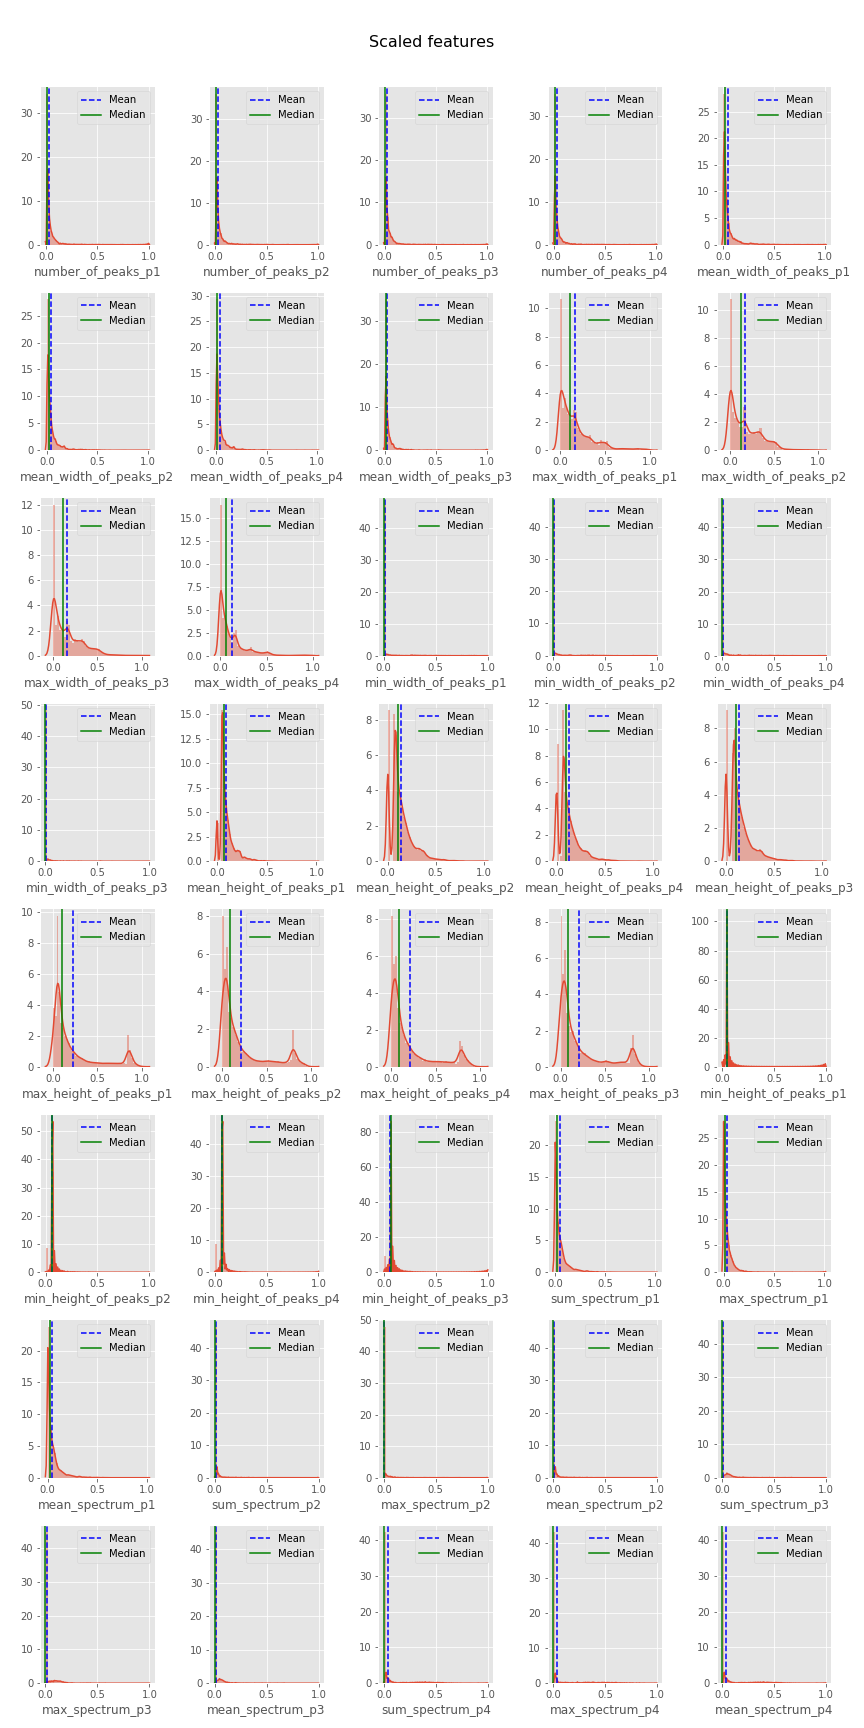
\includegraphics{dist_minmax_scaled.png}
\caption{Scaled Features}
\end{figure}

It can be seen that almost all features distribution are skewed, which
means the data does not follow a normal distribution. Therefore, the
natural logarithm transformation is applied to the dataset.

\begin{figure}
\centering
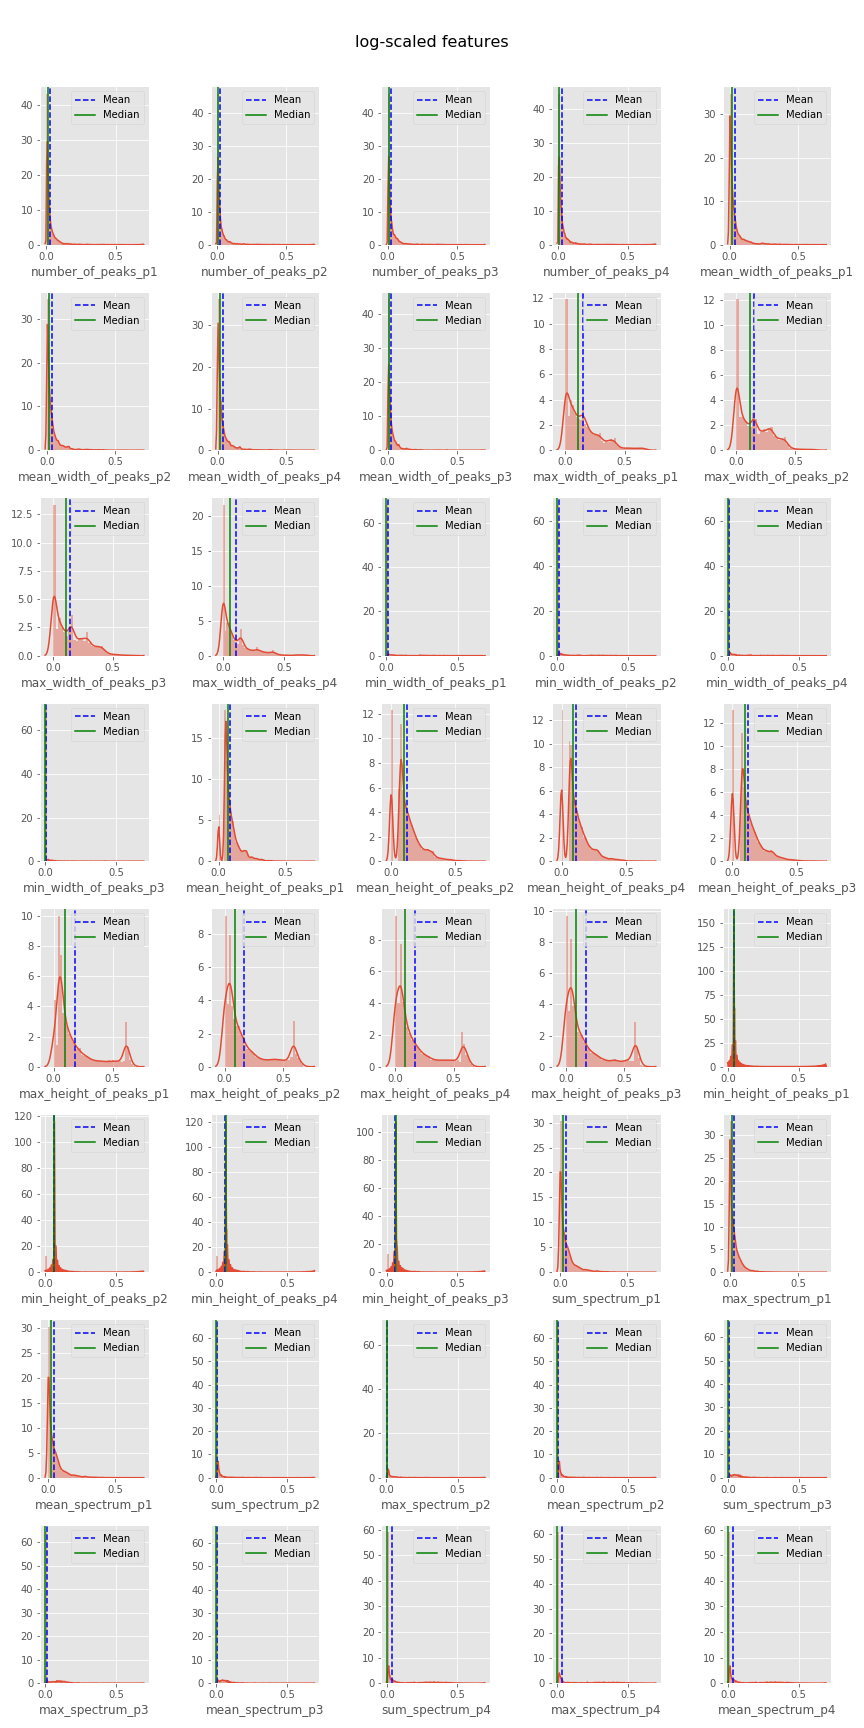
\includegraphics{dist_minmax_scaled_log.png}
\caption{Log-scaled Features}
\end{figure}

\hypertarget{feature-selection}{%
\paragraph{Feature Selection}\label{feature-selection}}

The next pre-processing step should be the feature selection using a
tree-based approach. The idea behind this is that in every node in a
decision tree is a condition is tested on a single feature, which is
called the impurity. Thus, when training a tree, we can calculate how
much each feature decreases the impurity in a tree. Finally, if we build
an ensemble of trees, we can average these values on different subsets
of the data and estimate the importance of the variables. For this task,
the
\href{https://scikit-learn.org/stable/modules/generated/sklearn.ensemble.ExtraTreesClassifier.html}{ExtraTreeClassifier}
model will be used.

After applying this feature selection algorithm to the dataset, the
importance of each feature can be seen in the figure below.

\begin{figure}
\centering
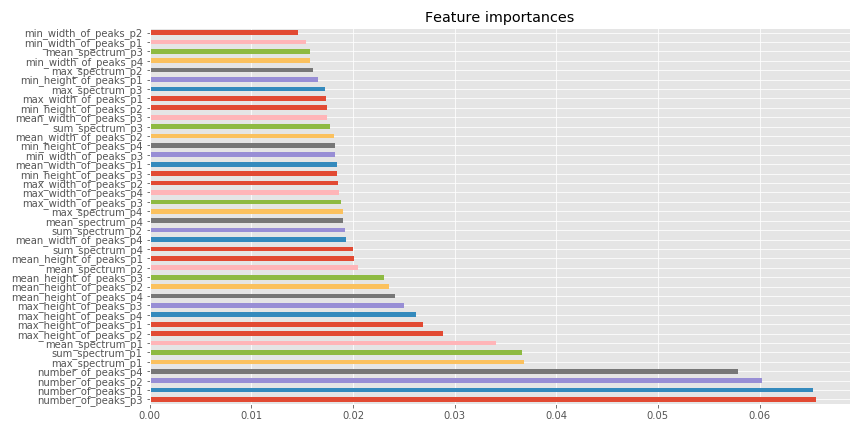
\includegraphics{feature_importances.png}
\caption{Feature Importance}
\end{figure}

Based on this result, the following features will be selected for
training the prediction models: \texttt{number\_of\_peaks\_p1},
\texttt{number\_of\_peaks\_p2}, \texttt{number\_of\_peaks\_p3},
\texttt{number\_of\_peaks\_p4}, \texttt{max\_height\_of\_peaks\_p1},
\texttt{max\_height\_of\_peaks\_p2},
\texttt{max\_height\_of\_peaks\_p4},
\texttt{max\_height\_of\_peaks\_p3}, \texttt{sum\_spectrum\_p1},
\texttt{max\_spectrum\_p1}, \texttt{mean\_spectrum\_p1}

\hypertarget{implementation}{%
\subsubsection{Implementation}\label{implementation}}

The implementation process starts by extracting the features for each
signal in the \texttt{train.parquet} file, as described before. Each
signal needs to be denoised and then the features can be extracted. The
signal denoising functions are in the \texttt{signal\_denoising.py} file
and the feature extraction in the \texttt{feature\_extraction.py} file.
This is the most time-consuming task, since each signal took around 0.5
seconds to be loaded and processed, thefore taking up to 1.2 hours to
process all the signals in the training dataset (8712). This was done in
the \texttt{execute\_signal\_processing.py} file, which will generate
the output file \texttt{all\_features.csv} with the extracted features.
Next, this file is loaded and the feature scaling, transformation and
selection are executed. This task, and the model learning are available
in the \texttt{data\_processing\_and\_modeling} Jupyter notebook.

The remaining process is very straightforward, and consists in the
following steps: * Load the dataset with the features already extracted
transformed and selected into memory * Split the dataset into training
(80\%) and test (20\%) sets * Evaluate several models using 10 fold
cross-validation on the training set * Select the trained model with the
highest MCC cross validation score * Train the selected model on
training set * Grid search will be used to select the optimal
hyperparameters * Evaluate the model MCC score on the test set

\hypertarget{refinement}{%
\subsubsection{Refinement}\label{refinement}}

As mentioned in the Benchmark section, the naive predictor achieved a
poor MCC score of \texttt{0.0}. To get an initial result, a few models
using default hyperparameters were tested agains the dataset: kNN,
Gradient Boosting, Random Forest and Logistic Regression. The results
can be seen on the boxplot below.

\begin{figure}
\centering
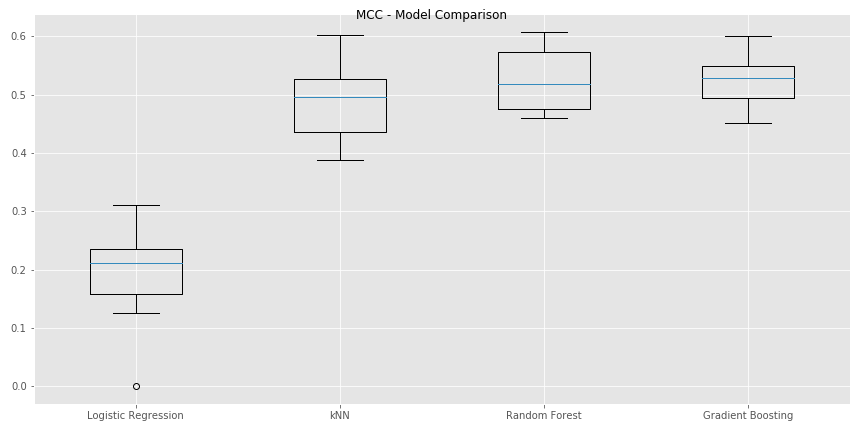
\includegraphics{model_cross_val_trial.png}
\caption{Model Cross-validation}
\end{figure}

We can see that all the proposed models achieved a better score than our
benchmark. Since the Random Forest model achieved a high score with only
10 trees in the forest, it will be selected as the model to be
optimized. The grid search algorithm will be executed on the following
hyperparameters configuration:

\begin{itemize}
\tightlist
\item
  \texttt{n\_estimators}: {[}10, 30, 50, 100, 150, 200, 300{]}
\item
  \texttt{max\_features}: {[}`auto', `sqrt'{]}
\item
  \texttt{max\_depth}: {[}10, 30, 50, 70, 100, None{]}
\item
  \texttt{min\_samples\_split}: {[}2, 5{]}
\item
  \texttt{min\_samples\_leaf}: {[}1, 2, 4{]}
\end{itemize}

After executing the Grid Search for every combination of these
parameters, the optimal model achieved a MMC score of \texttt{1.0} on
the training set and \texttt{0.6} on the test set.

    \hypertarget{iv.-results}{%
\subsection{IV. Results}\label{iv.-results}}

\hypertarget{model-evaluation-and-validation}{%
\subsubsection{Model Evaluation and
Validation}\label{model-evaluation-and-validation}}

The final optimal hyperparameters for the random forest classifier are
summarized below:

\begin{itemize}
\tightlist
\item
  \texttt{n\_estimators}: 200
\item
  \texttt{max\_features}: `auto'
\item
  \texttt{max\_depth}: 30
\item
  \texttt{min\_samples\_split}: 5
\item
  \texttt{min\_samples\_leaf}: 1
\end{itemize}

The model was chosen because it achieved the highest MCC score in the
training data. The hyperparameters are also very reasonable, not having
any very extreme values selected. To verify the robustness of the final
model, the test data was evaluated, achieving a MCC score was
\texttt{0.6}, which is a good value. However, it suggests that there was
some overfitting on the training data, since the training score was
\texttt{1.0}.

\hypertarget{justification}{%
\subsubsection{Justification}\label{justification}}

Comparing to the benchmark model, the final solution was much better.
The test MCC score values was increased from \texttt{0} to \texttt{0.6},
achieving the objective of this project. The figure below displays the
confusion matrix of the test set evaluations.

\begin{figure}
\centering
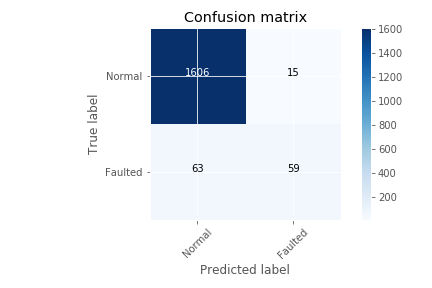
\includegraphics{cnf_matrix_testset.png}
\caption{Confusion Matrix}
\end{figure}

The analysis of the confusion matrix shows that the model did a very
good job classifying the normal signals. Its biggest challenge was to be
able to correclty classify the faulted signals: only 48\% of the
examples were correctly classified as faulted, which was the reason the
MMC score was not very high. This could be an effect of the very
unbalanced dataset.

The model was also evaluated against Kaggle's test set, achieving a
score of \texttt{XXX}. This placed me among the top XX competitors, as
of February 4th.

    \hypertarget{v.-conclusion}{%
\subsection{V. Conclusion}\label{v.-conclusion}}

\hypertarget{free-form-visualization}{%
\subsubsection{Free-Form Visualization}\label{free-form-visualization}}

The biggest challenge of this project is to find a representation of the
PD signal that is good enough to separate between a faulted and normal
signal. The figure below shows an example of signals classified as
faulted and normal.

\begin{figure}
\centering
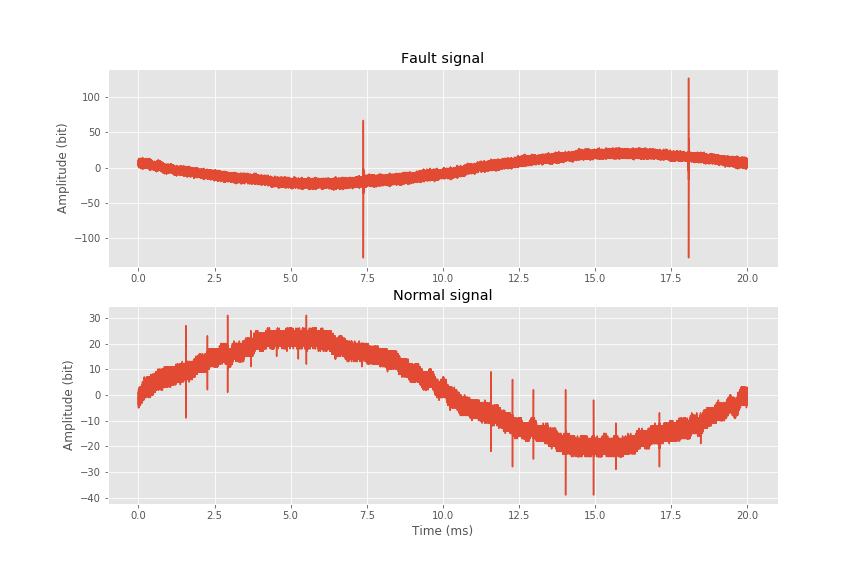
\includegraphics{signal_fault_normal_raw_freeform.png}
\caption{Fault and normal signals}
\end{figure}

Visually, it is pratically impossible to classify each signal. In fact,
the faulted signal has less peaks and is less noisy than the regular
one! However, after applying feature extraction and data pre-processing
techniques, it was possible to find relevant features that are able to
separate them. This also summarizes a very interesting and exciting
characteristic of this dataset: how a signal having 800,000 samples can
be represented by only 11 features and be correclty classified only with
this information. Furthermore, it higlights the importance of the data
pre-processing in any data science project.

\hypertarget{reflection}{%
\subsubsection{Reflection}\label{reflection}}

The process used for this project can be summarized using the following
steps:

\begin{enumerate}
\def\labelenumi{\arabic{enumi}.}
\tightlist
\item
  An interesting and relevant problem with public data sets was found
\item
  The data was downloaded, the signals denoised and the features
  extracted
\item
  A benchmark was created for the classifier
\item
  Several classifiers were evaluated and the best one selected
\item
  The selected classifier was trained using the available train data,
  using grid search to optimize the hyperparameters
\item
  The test data was evaluated against the optimal classifier
\item
  The model predictions were submitted to the Kaggle website
\end{enumerate}

Step 2 was the most difficult and time-consuming task, because in order
to correctly define the denoising and feature extraction techniques I
had to study the available literature on PD signal processing. Since I
already had a good background on the problem domain, I knew where to
seek the necessary information and this became a very straight-forward
task, even though being quite complex. I also decided to spend more time
studying the feature selection and transformation, in order to polish my
skills on these tasks and also produce a final dataset with better
quality. In fact, this was the most interesting and important step in
the project, since I could effectively see the impact of a good data
preparation step on the model learning.

Steps 4 and 5 took less time than expected, since my choice of features
proved to be good and the models achieved better results than the
benchmark on the first trials.

\hypertarget{improvement}{%
\subsubsection{Improvement}\label{improvement}}

To achive better results, I believe the first step is trying to improve
the quality of the PD denoising and feature extraction algorithms. In
{[}1{]}, the author presents a series of signal representation
techniques that can be used to extracted more relevant features from the
PD signals. There are also a very large literature on PD denoising
techniques, which could also be explored. Due to their complexity and
the project's time constraints, I decided to only use the denoising and
feature extraction techniques I was most familiar with.

As for the models improvements, I believe it is worth exploring more the
Gradient Boosting algorithm, since it also achieved good results on the
initial trial and also works very well in practice. This could improve
the overfitting observed on the training dataset and improve the current
benchmark with random forests.

    \hypertarget{references}{%
\subsubsection{References}\label{references}}

{[}1{]}
http://dspace.vsb.cz/bitstream/handle/10084/133114/VAN431\_FEI\_P1807\_1801V001\_2018.pdf

{[}2{]} S. Sriram, S. Nitin, K.M.M. Prabhu, and M.J. Bastiaans. Signal
denoising techniques for partial discharge measurements. IEEE
Transactions on Dielectrics and Electrical Insulation, 12(6):1182--1191,
2005

{[}3{]} Ma, X., Zhou, C. and Kemp, I.J., 2002. Interpretation of wavelet
analysis and its application in partial discharge detection. IEEE
Transactions on Dielectrics and Electrical Insulation, 9(3), pp.446-457.

{[}4{]} S. Misák, J. Fulnecek, T. Vantuch, T. Buriánek and T. Jezowicz,
``A complex classification approach of partial discharges from covered
conductors in real environment,'' in IEEE Transactions on Dielectrics
and Electrical Insulation, vol.~24, no. 2, pp.~1097-1104, April 2017.

{[}5{]} Liaw, A. and Wiener, M., 2002. Classification and regression by
randomForest. R news, 2(3), pp.18-22.


    % Add a bibliography block to the postdoc
    
    
    
    \end{document}
